%!TEX TS-program = pdflatex
\documentclass[letterpaper, 10 pt, conference]{ieeeconf}  % Comment this line out if you need a4paper

%\documentclass[a4paper, 10pt, conference]{ieeeconf}      % Use this line for a4 paper

\IEEEoverridecommandlockouts                              % This command is only needed if 
                                                          % you want to use the \thanks command

\overrideIEEEmargins                                      % Needed to meet printer requirements.

% See the \addtolength command later in the file to balance the column lengths
% on the last page of the document

% The following packages can be found on http:\\www.ctan.org
\usepackage{color}
\usepackage{graphics} % for pdf, bitmapped graphics files
\usepackage{epsfig} % for postscript graphics files
%\usepackage{mathptmx} % assumes new font selection scheme installed
%\usepackage{times} % assumes new font selection scheme installed
\usepackage{amsmath} % assumes amsmath package installed
\usepackage{amssymb}  % assumes amsmath package installed
\usepackage{subfigure}
\usepackage{url}

\renewcommand{\baselinestretch}{0.91}
\hyphenation{methodo-logy}

% \addtolength{\topmargin}{50pt}
\title{\LARGE \bf Soft-Actuators in Cyclic Motion: Analytical Optimization of Stiffness and Pre-Load 
}

\author{Alexandra Velasco$^*$, Gian Maria Gasparri$^\dagger$, Manolo Garabini$^*$, Lorenzo Malagia$^*$, \\Paolo Salaris$^*$ and Antonio Bicchi$^{*\dagger}$
\thanks{The research leading to these results has received funding from the European Union Seventh Framework Programme   under grants FP7 ICT-287513 ``SAPHARI'' project and the ERC Advanced Grant 291166 ``SoftHands'' project.}
\thanks{$^*$ Research Center ``Enrico Piaggio'', University of Pisa, via Largo Lucio Lazzarino, 1, 56126 Pisa, Italy.}
\thanks{$^\dagger$ Department of Advanced Robotics, Istituto Italiano di Tecnologia, via Morego, 30, 16163 Genova, Italy}
}

\begin{document}


\maketitle
\thispagestyle{empty}
\pagestyle{empty}


%%%%%%%%%%%%%%%%%%%%%%%%%%%%%%%%%%%%%%%%%%%%%%%%%%%%%%%%%%%%%%%%%%%%%%%%%%%%%%%%
\begin{abstract}
In this paper, we study the role of soft actuation in the reduction of the energy cost for mechanical systems that perform cyclic tasks. The objective is to determine the optimal stiffness value and spring pre-load such that a given cost functional is minimized. For the analysis, we consider both fully actuated and underactuated mechanical systems using elastic actuators which, depending on how and where the springs are placed w.r.t.~the actuator and the load, can be Series Elastic Actuators (SEAs) or Parallel Elastic Actuators (PEAs). The energy consumption depends not only on the actuation parameters but also on the trajectories followed to perform a given cyclic task. We show that the general problem in which both joint trajectories and actuation parameters are the optimization variables, can be cast as a simpler problem in which optimization regards only joint trajectories. Simulations of fully actuated and underactuted compliant robots are reported to demonstrate the effectiveness of the method.
Although the stiffness optimization method is analytical in nature, it is directly applicable to existing systems whose model is unknown. A model--free experimental application on a prototype of a hopping robot with SEA is presented.
\end{abstract}


%%%%%%%%%%%%%%%%%%%%%%%%%%%%%%%%%%%%%%%%%%%%%%%%%%%%%%%%%%%%%%%%%%%%%%%%%%%%%%%%
%!TEX root = Humanoids2013.tex
\section{Introduction}
\label{sec:introduction}

A crucial component that dramatically affects performance of robots is their actuation. Recent developments in this field have introduced fixed or physically adjustable compliant elements to enrich the dynamics of conventional motors. %\cite{SoftRoboticsDLR08, TsLaVaCa09}.%  (see SMART ACTUATORS and REVIEW VSA)
These devices provide advantages w.r.t.~rigid actuators, including higher peak performances, lower energy consumption and improved safety (see \cite{Pratt95,VanderborghtVHDLDB06,CGGBMTB11}, \cite{Taylor:2011}). This new tendency is the so called soft actuation, used for instance in manipulation \cite{SoftRoboticsDLR08}, or in humanoid design \cite{TsLaVaCa09}.

Among soft actuators, SEAs~\cite{Pratt95} have a linear compliant element between a high impedance actuator and the load. On the other hand, PEAs have an elastic element in parallel with the motor (i.e. between two links). Other examples of soft actuators are the Variable Stiffness Actuators (VSA), and the Variable Impedance Actuators (VIA). VSAs have an elastic transmission whose stiffness can be mechanically adjusted, while VIAs can include mechanisms (e.g.~brakes, dampers) allowing to change the output shaft impedance~\cite{CGGBDBTB12:2}.
% 
%  have a elastic element in series between the motor and the load. The latter allows also to change the motor's damping . 
Recent studies explore the role of such devices in performance enhancement, looking at very dynamic tasks. For instance, in \cite{AlbuSchaffer2011, Garabini2011} the objective is to optimally choose the stiffness to maximize the velocity of a VSA at a given final position with free final time. In \cite{CGGBDBTB12}, a new constraint is imposed, solving the same problem but with fixed terminal time.
% VSA VIJAYKUMAR %\cite{ViHo11}
% Optimal control is also addressed in \cite{nakanishi11} to achieve efficient actuators and control of a periodic motion for dynamical systems by exploiting intrinsic passive dynamics of VSA. %The methodology presented has not been applied to systems as walking or hopping robots. 
% One of the goals of humanoid robotics is to understand human dynamics as well as to reproduce it in simulation and hardware. However, SEA are non-commercial, and this means that most of them have been designed for specific applications \cite{Taylor:2011}, \cite{doi:10.1117/12.548000}. 
% Among the robots that use compliant actuation, \cite{4115608}, \cite{620132}, \cite{4115646}, \cite{MABEL}, \cite{4115607}, \cite{VanderborghtVHDLDB06}, \cite{ZVTCC2012}, for example in \cite{4115608} the compliance is tuned to have natural motion of the legs.
% In \cite{Hurst08} a monopod leg is presented with the knee joint actuated by a SEA. Experimental tests have shown that a suitable stiffness value reduces the mechanical work done by the motor during a stance phase while hopping in place.
% Motivations that pushed the development toward this direction arise in the intent of the robotics community to give humanoid robots the best characteristics of human beings. In fact, humans are low stiffness, low bandwidth systems (TODO cite), compared to most of the humanoid robots designed that have high bandwidth, and which are stiff \cite{Pratt95}, \cite{4115607}. 
 
\begin{figure}[t!]
\centering
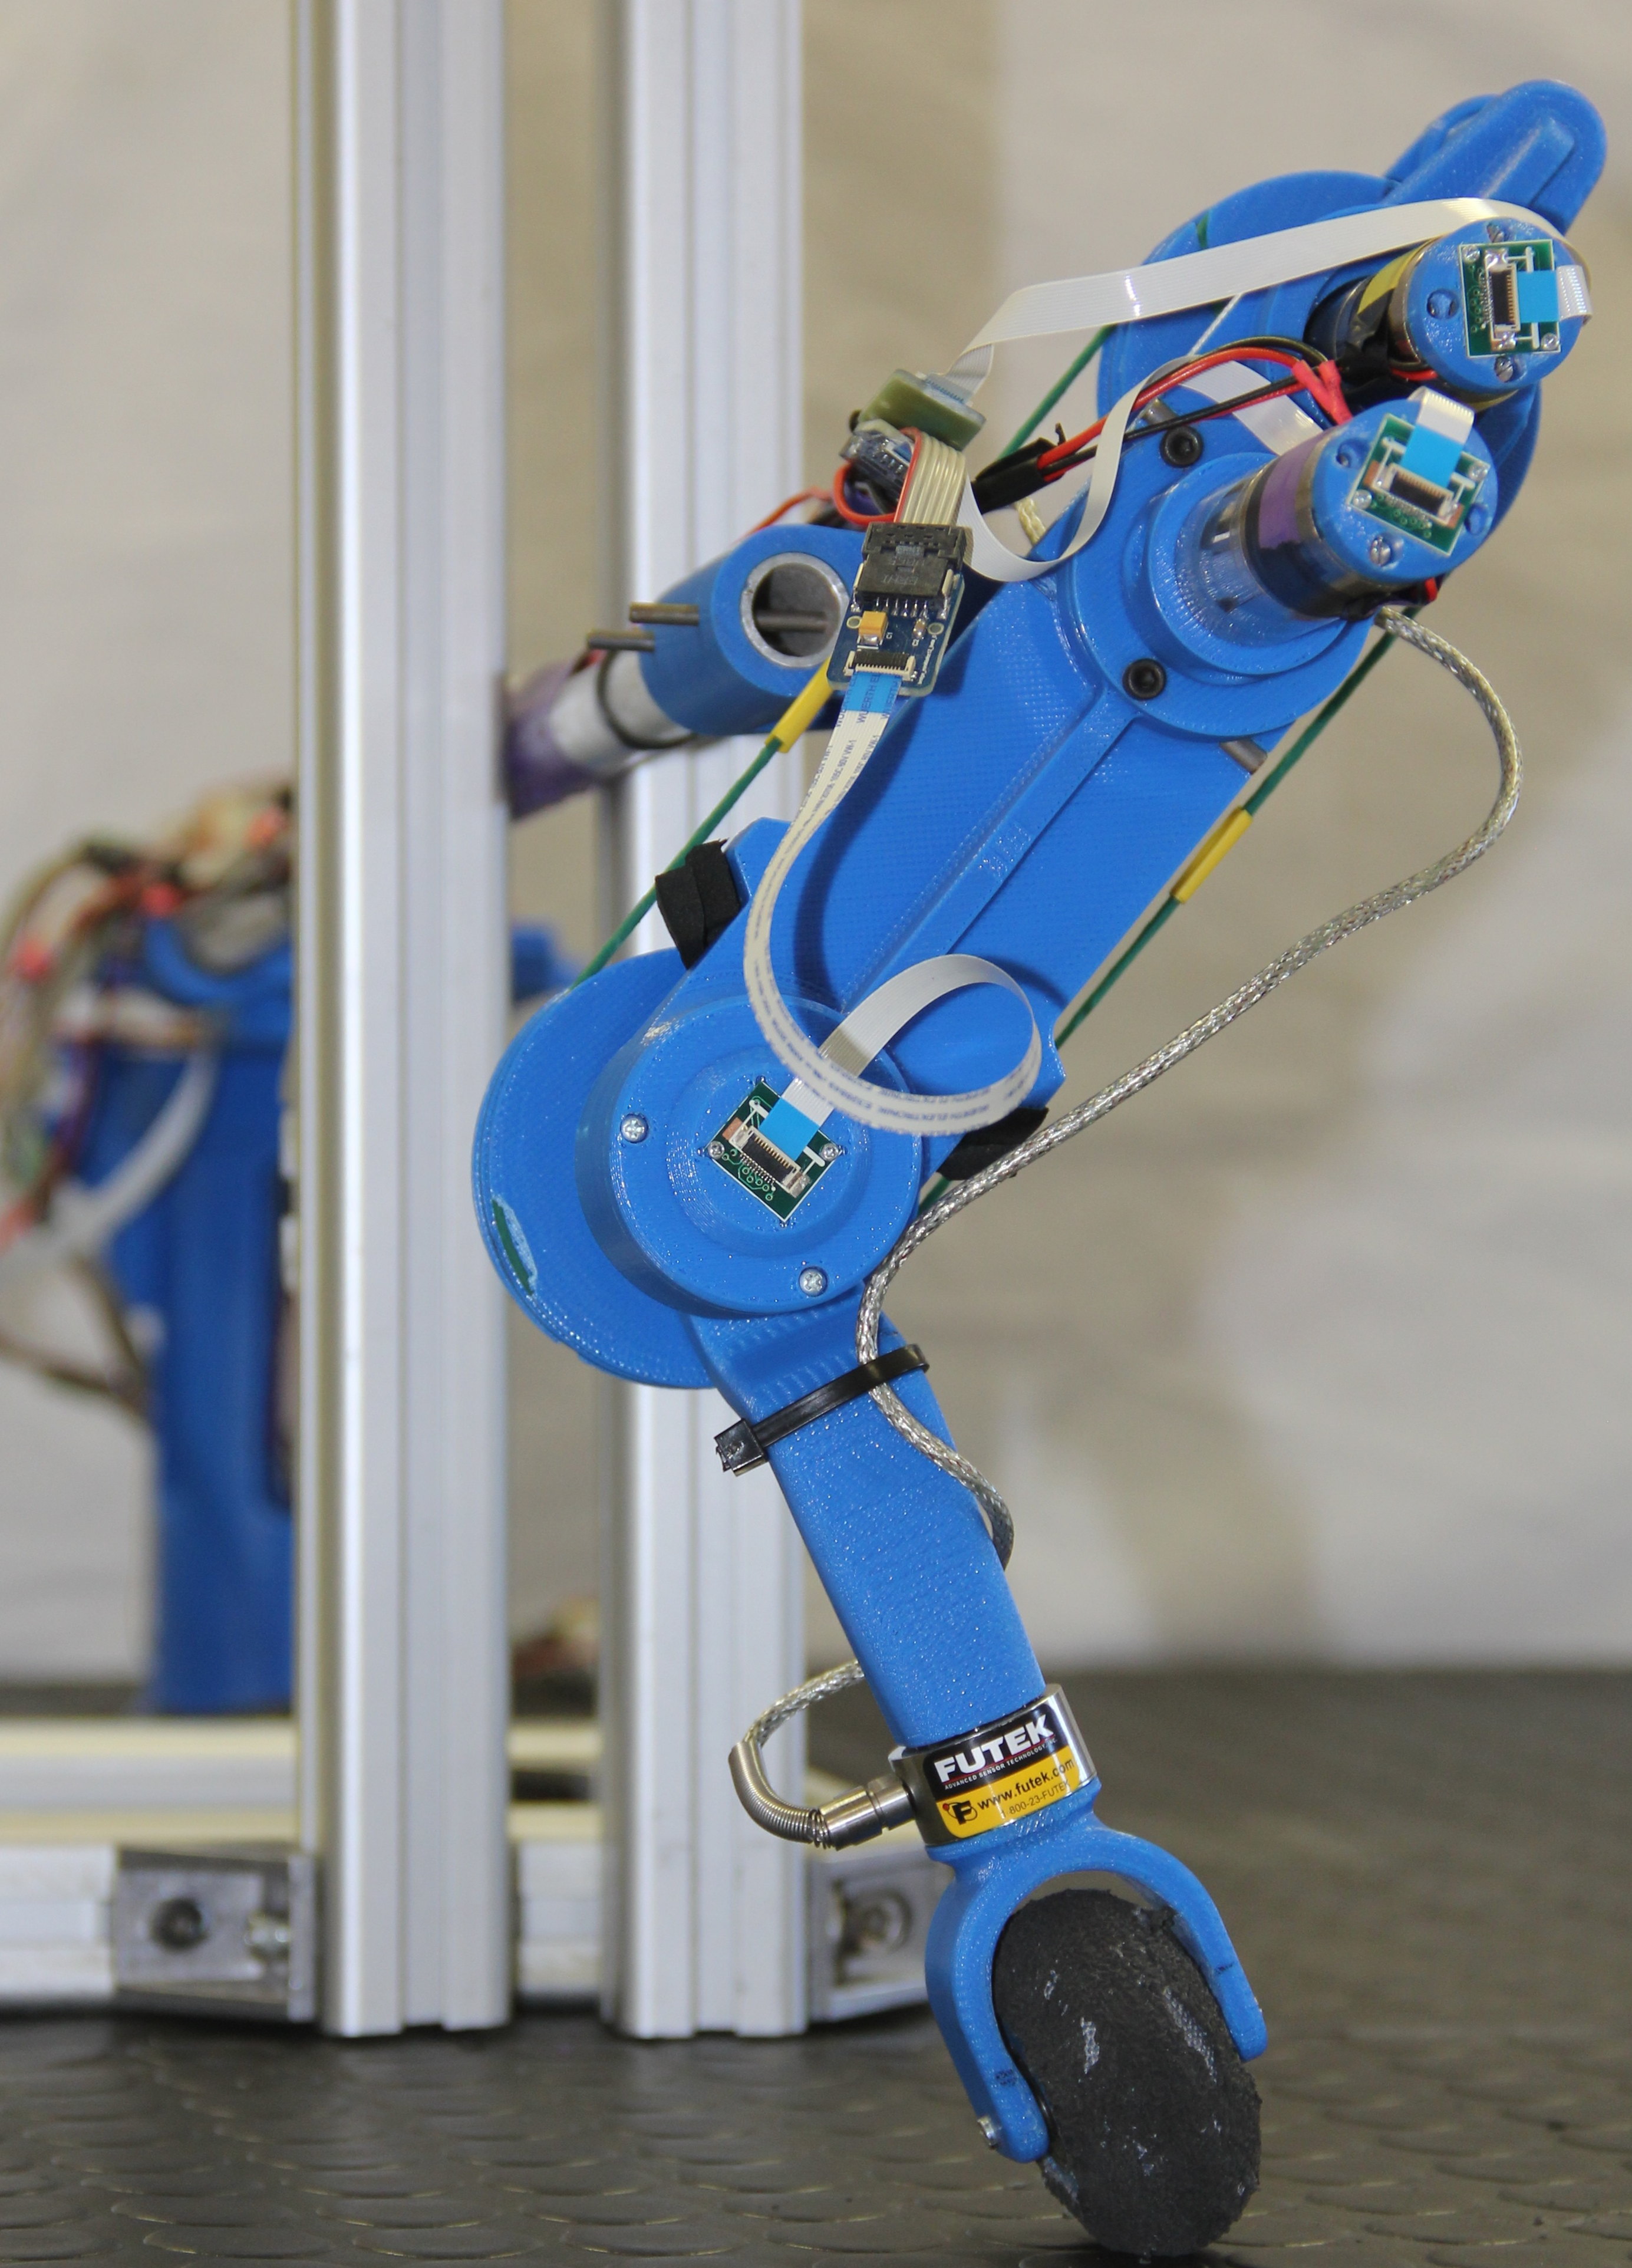
\includegraphics[width=0.7\columnwidth]{dwg/Saltarello}
\caption{The prototype of the Hopper used for experiments.}
\label{fig:Prototype}
\end{figure}
In this paper, we study the role of soft actuation in the reduction of the energy cost for mechanical systems that perform cyclic tasks. The objective is to determine, for given desired joint trajectories, the optimal stiffness value and spring pre-load such that a given cost functional is minimized.

% Fully actuated and underactuated dynamical systems using elastic actuation are considered. % Paragraph in which robots energy efficiency statistics 
% An analytical methodology to optimize the actuation parameters (joint stiffness and pre-load, the first in the SEA case or both in the PEA case), for given joint trajectories, is presented. 
% The method can be applied using different performance indices (based on squared torque, or squared mechanical power) to be chosen on the basis of the type of actuation. 
% Moreover, this work, holds up that the performance index depends on the desired joint trajectories as well as on the actuation parameters. 
% With the presented methodology, the general problem in which both joint trajectories and actuation parameters have to be simultaneously optimized, can be translated into a problem in which the optimization involves just the joint trajectories.
%In this work it is shown that he performance index also depends on the desired joint trajectories; therefore this methology is extended to find the optimal joint trajectories by solving a nonlinear optimization problem subject to constraints that depend on the dynamics and on the desired task.  
 % Finally, a planar model of a biped robot that includes the trunk is considered. %In this case, the optimal stiffness for each joint which minimizes its energy consumption for a given walking gait is found. 
% For measuring the performance we define the Cost of transport (CoT) as in \cite{MSTLDS2010}. This cost measures the specific mechanical energy spent by the actuators divided by the mass and the traveled distance. The mechanical energy is considered as the time integral of the absolute value of the power spent by the actuators. This definition assumes that the negative work of an actuator cannot be used and that no brake is present, so the negative work must be produced by the actuators. For the examples presented, the cycles have been selected to have a known behavior of the system. Applying the proposed method, the elastic constant for each joint are found.

In the literature, several papers try to solve the same problem addressed in this work. 
%%%%%%%%%%%%%%%%%%%%%%%%%%%%%%%%
%NIKOS ICRA '13
For instance, a systematic method to optimally tune the joint stiffness of multi Degrees of Freedom (DoFs) SEA robots based on resonance analysis and energy storage maximization criteria is presented in \cite{Nikos13}. A modal study was performed on the CoMAN (Compliant huMANoid) robot model, to derive the natural frequencies for different leg configurations during the single support walking phase. The joint stiffness was selected to set the resonances of the system, 
% by solving a constrained optimization problem with a cost function that 
maximizing the energy stored in the joint springs. 
% of the robot or the joint passive deflection for a given joint torque vector. 
% Moreover, authors consider to set joint stiffness for the walking robot, though 
However, in \cite{Nikos13}, the design of trajectories is not based on joint stiffness selection directly and an approach to find the optimal stiffness and pre-load for the PEA case has not been addressed yet. 
% In \cite{MSTLDS2010} the performance of a passive-dynamic swinging leg is shown through the evaluation of energy efficiency. The joint trajectories are not derived in the mentioned work, though the passive joint stiffness is used to reduce the energetic cost in the swing phase (in walking).
Walking gaits generation for biped robots has also been addressed as a nonlinear optimization problem in~\cite{Ott12}. The trajectories are obtained through cubic spline interpolation but joint compliance is not considered. In~\cite{Ting10}, an optimization is proposed to find feasible trajectories for a hopping robot. By constraining the problem, stable hopping of the rigid, underactuated robot is achieved.  

A control method for tracking cyclic trajectories is presented in~\cite{Kawamura09:2}, taking advantage of resonance of the dynamic systems and hence obtaining the optimal (constant, linear) stiffness value.  
In~\cite{Kawamura09:1} an energy saving control method was applied to a simulated biped walking model. The link trajectories for a 4 DoF PEA robot are obtained via minimization of a performance index based on the squared torque. However, as in~\cite{Kawamura09:2}, the SEA case is not considered. 

In this paper, we consider both fully actuated and underactuated dynamical systems using elastic actuation with either SEA or PEA providing an analytical methodology to optimize the actuation parameters for given joint trajectories. We show that the general problem in which both joint trajectories and actuation parameters have to be simultaneously optimized, can be translated into a problem in which the optimization would involve just the joint trajectories. However, in this paper the optimal characterization of the joint trajectories shape is not considered, showing only that, in case of sinusoidal trajectories the amplitude and the frequency play an important role in the reduction of the energy spent.

To show the effectiveness of the results we apply our method to a simple one-link robot manipulator tracking a sinusoidal joint trajectory and to a two-link robot manipulator performing a pick and place task. 
By several simulations, in both cases we show that the use of soft actuation allows to save energy w.r.t.~the stiff actuation case. For the pick and place task, optimized soft actuation allows to save up to 53\% of energy. 
% To show insights and application of the results of this paper we report three examples. First we briefly present the SEA one-DoF case study with a sinusoidal desired trajectory. For this problem the proposed method provides the stiffness that makes the natural frequency of the system equal to the frequency of the desired trajectory. 
% Then we present the case of two-DoF manipulator with SEA which performs a pick and place task. We will show that, in the best case, optimized soft actuation allows to save the XX\% of the total mechanical energy w.r.t. rigid actuation.
Finally, a prototype of a hopping robot with SEAs is presented (see Fig.~\ref{fig:Prototype}) and by experimentation we show that our method is applicable to existing systems whose model is unknown.

%!TEX root = Humanoids2013.tex
\section{Problem Definition}

This paper considers novel soft-robotics actuation schemes which may enhance performance of mechanical systems in cyclic tasks, i.e.~reducing energy consumption, by exploiting the use of springs suitably placed on the system. For this reason, we study compliant mechanical systems which can be both fully actuated or underactuated. In the former case, there are as many actuators as Degrees of Freedom (DoF), whereas in the second one there are fewer control inputs than degrees of freedom~\cite{spong98}. 

Depending on how and where springs are placed on the system, the number of DoFs and the number of actuators, the dynamics of a mechanical system can assume particular forms as described in next subsections.

% An optimization method has been proposed to find the best actuation parameters for fully actuated and underactuated robots.  
% %The cost function and the index to minimize are based on the resulting motor torques and velocities.
% 
% Commonly underactuated mechanical systems are those mechanical systems that have fewer control inputs than degrees of freedom \cite{spong98}. In our work the underactuated mechanical systems denote the systems that have fewer actuator than degrees of freedom, whatever the nature of actuation is. As a consequence, the fully actuated systems are those systems that have as many actuators as degrees of freedom.
% We are particularly interested in studying compliant systems.

\subsection{Fully Actuated Mechanical Systems}
\label{sec:FullyActuatedSystems}

Let us first consider a fully actuated compliant mechanical system actuated by PEAs, e.g.~a spring between two links for a serial manipulator (see Fig.~\ref{fig:PEA}). For such a system, the number of DoFs remains equal to the number of actuators. Indicating by $q\in\Re^n$
the generalized coordinates representing the configuration of the system and by $\tau\in\Re^n$ the generalized torque provided by actuators, the dynamics can be written as
\begin{equation}
\label{eq:FullyActuated}
f(\ddot q,\dot q, q, t)=-K(q_e-q)+\tau\,,
\end{equation}
where $q_e\in\Re^n$ is the spring pre-load and $K\in\Re^{n\times n}$ is the stiffness matrix. The term $f(\ddot q,\dot q, q, t)$ includes inertia, coriolis, and gravity terms.
\begin{figure}[!t]
\centering
\subfigure[Example of robot actuated by PEA.]{\label{fig:PEA}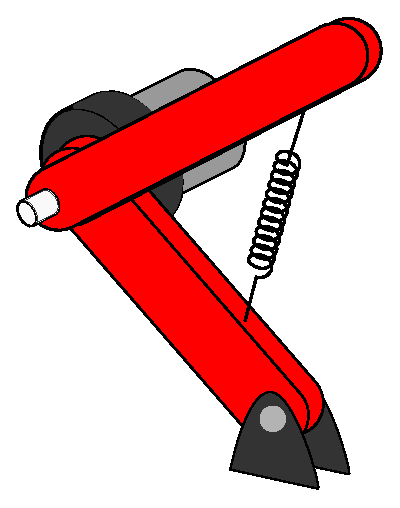
\includegraphics[width=0.25\columnwidth]{dwg/PEA}}
\quad
\subfigure[Example of robot actuated by SEA.]{\label{fig:SEA}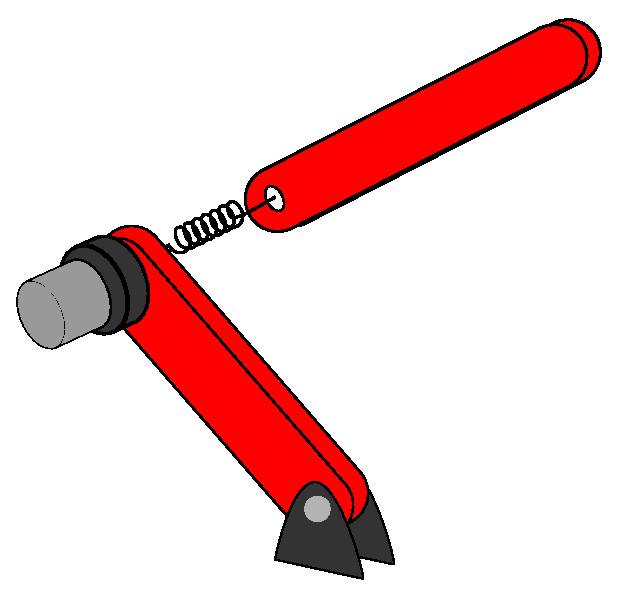
\includegraphics[width=0.4\columnwidth]{dwg/SEA}}
% 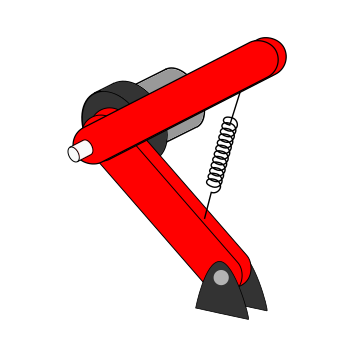
\includegraphics[width=0.4\columnwidth]{PEA}
\caption{Robot actuated by PEAs or SEAs.}
\label{fig:PEA_SEA}
\end{figure}

\subsection{Underactuated Mechanical Systems}
\label{sec:UnderActuatedSystems}

Consider now the case in which the mechanical system is actuated by SEAs (see Fig.~\ref{fig:SEA}), i.e.~the springs between the actuator and the load (e.g.~between the motor and the link for serial manipulators). Indicating by $\theta\in\Re^n$ the motor positions and by $J_m$ the inertia matrix of the motors, the dynamics can be written as
\begin{align}
\label{eq:actuated1_SEA}
f(\ddot{q}, \dot{q}, q, t) &= - K(q - \theta) \\
J_{m} \ddot{\theta} &= K(q - \theta) + \tau\,,
\label{eq:actuated2_SEA}
\end{align}
Notice that the use of SEAs instead of PEAs increases the number of DoFs which become $2n$. 

For particular mechanical systems there may be further DoFs which are not actuated, e.g.~the position and orientation of humanoids w.r.t. a fixed reference frame. Let $x\in\Re^m$ be those DoFs and assume the system is actuated by SEAs, the dynamics in this case can be written as 
\begin{align}
\label{eq:noact_SEAplus}
f_u(\ddot x, \dot x, x, \ddot{q}, \dot{q}, q, t) &= 0  \\
\label{eq:underact1_SEAplus}
f_a(\ddot x, \dot x, x, \ddot{q}, \dot{q}, q, t) &= - K(q - \theta)  \\
J_{m} \ddot{\theta} &= K(q - \theta)+\tau,
\label{eq:underact2_SEAplus}
\end{align}
where~\eqref{eq:noact_SEAplus} represents the non-actuated dynamics, whereas~\eqref{eq:underact1_SEAplus} and \eqref{eq:underact2_SEAplus} represent the underactuated dynamics.

Of course, if PEAs are used, the dynamics becomes
\begin{align}
\label{eq:noact_PEAplus}
f_u(\ddot x, \dot x, x, \ddot{q}, \dot{q}, q, t) &= 0  \\
\label{eq:underact_PEAplus}
f_a(\ddot x, \dot x, x, \ddot{q}, \dot{q}, q, t) &= - K(q_e - q)+\tau\,.
\end{align}
% \subsection{Fully Actuated Systems}
% 
% The general dynamics model of a n-DoF fully actuated system, using series elastic actuators can be written as 
% \begin{equation}
% f(\ddot{q}, \dot{q}, q, t)= - K(q - \theta)  
% \label{eq:actuated1}
% \end{equation}
% \begin{equation}
% J_{m} \ddot{\theta} - K(q - \theta) =  \tau,
% \label{eq:actuated2}
% \end{equation}
% where $f \in\Re^{n\times 1}$ is the dynamics expression of the system, which includes the inertia terms, the coriolis terms, and the gravity terms. 
% $q \in\Re^{n}$ is the vector of desired trajectories for each link, $\theta \in\Re^{n}$ is the vector of motor positions.
% $K \in\Re^{n\times n}$ is the elastic elements matrix, and $J_{m} \in\Re^{n \times n}$ is the motor's inertia matrix.
% $\tau \in \Re^{n}$ is the actuators torque.  
% 
% For n-DoF fully actuated systems with parallel elastic actuation, the dynamics model is
% \begin{equation}
% f(\ddot{q}, \dot{q}, q, t)= - K(q_e - q) + \tau \, ,  
% \label{eq:actuatedPEA}
% \end{equation}
% where $q_e \in \Re^{n}$ is the actuator pre-load.  

%%%%%%%%%

\subsection{Optimal Problem Formulation}

In order to quantify the performance of the mechanical system and hence to determine optimal joint stiffness $\hat K$ and/or pre-load $\hat q_e$ values as well as optimal joint trajectories $q(t)$, we will consider two different cost functionals:

\subsubsection{Squared-Power index}
Assuming that the motor spends energy if the mechanical power is positive or negative, the cost functional of the whole mechanical system is 
\begin{equation}
	J_1 = \sum_{j=1}^{n} \int_0^T(\tau_{j}(t)\dot{\theta_{j}}(t))^2dt\,,
\label{eq:J2}
\end{equation}
where $T$ represents the period of the cyclic task or its multiple. %energy spent by each actuator to accomplish the desired task: 
%\begin{equation}
%	J_1 = \sum_{j=1}^{m} \int_0^T{(\tau_{j}\dot{\theta_{j}}(t))dt}\, ,
%	\label{eq:J1}	
%\end{equation}

%This index serves if the actuators can store energy when the mechanical power is negative. Nevertheless, non back-drivable motors spend energy when its mechanical power is positive and when it is negative. Then, a more suitable performance index will be \eqref{eq:J2}:
 
% Then, the total performance index to minimize will be the sum of the joint costs 
% 
% \begin{equation}
% J_{1} = \sum_j{J_{1,j}} \,.
% \label{eq:ind1_gen}
% \end{equation}


\subsubsection{Squared-Torque index}
If the consumption is mainly related to the torque, then we can consider the cost
\begin{equation}
 J_2 = \sum_{j=1}^{n}\int_{0}^{T}{\tau_j^2 (t) dt}\,.
\label{eq:J3}
\end{equation}
% 
% \noindent then, the performance index is
% 
% \begin{equation}
% J_{2} = \sum_j{J_{2,j}} \,.
% \label{eq:ind2_gen}
% \end{equation}

% \subsection{Optimal trajectories problem formulation}
The optimal problem we are interested to solve is stated as follows: 
% The performance indices proposed depend also on the joint trajectories. Then, the optimization problem is stated as follows: 
\begin{equation} 
\begin{aligned}
\min_{\tau(t), \beta}{J_i},&\qquad i=1,2\\
s.t. & \\
& \begin{cases}  
  \text{Dynamics equations} \\
  q(t)=q(t+T)  \\
  \xi_1(q,\dot q,\ddot q)\leq 0 \\
  \xi_2(q,\dot q,\ddot q) = 0 \\
  \beta_m\leq \beta \leq \beta_M 
\label{eq:problem_form}
\end{cases}
\end{aligned}
\end{equation}
where the dynamic equations can be those reported in subsection~\ref{sec:FullyActuatedSystems} in case of a fully actuated system with PEAs or those reported in subsection~\ref{sec:UnderActuatedSystems} for an underactuated system with SEAs or PEAs. $\beta$ is a vector containing joint stiffness $K$ and pre-load $q_e$ in case of PEAs and only stiffness $K$ in case of SEAs. These values have limits $\beta_M=[K_M,\,q_{e,M}]$ and $\beta_m=[K_m,\,q_{e,m}]$. $T$ is the period of the cyclic task which translates in requiring that $q(t)=q(t+T)$. Moreover, the nonlinear constraints $\xi_1$ and $\xi_2$ which depend on variable $q$, $\dot q$ and $\ddot q$, define the task. For instance, in a pick and place task for a two-link planar manipulator, we can constrain the motion of the end-effector to the line between two points. 

% In this section, we consider how to reduce the energy consumption in cyclic tasks by optimally choosing joint stiffness values if the system is actuated by SEAs, and both joint stiffness and pre-load values in case of PEAs. Moreover, for a given ciclic task (e.g.~pick and place for a serial arm), we also show that the choice of the joint trajectories affects the performance of the system and we propose a methodology to determine the optimal trajectory.


%The minimization problem to solve, in order to find a feasible cycle for the leg hopping motion, is a nonlinear, constrained optimization problem, that can be solved numerically using MATLAB\textregistered  \textit{fmincon} function. The performance index \eqref{eq:J3} is the function that will be minimized, to find the $q$ trajectory that spends less energy, subject to the following constraints.

%%%%%%%%%%%%%%%%%%%%%%%%%%%%%%%%%%%%%%%%%%
%!TEX root = Humanoids2013.tex
\section{Optimization of Stiffness and Pre-Load parameters}
\label{sec:optimization}

% For illustrating the application of the method, we consider two general cases: a fully actuated system (n-DoF manipulator) and an underactuated system (n-link biped robot). One of the cases is studied using SEA and the mechanichal energy-based performance index and the other one using PEA and the torque based index; however, the method can be applied to general n-DoF fully actuated or underactuaded systems minimizing either one of the proposed indices.   
In this section we will exploit the dynamic equations of the mechanical system at hand in order to write the cost functional as a function of joint trajectories $q(t)$ (and their derivatives) and actuation parameters $\beta$. It is important to note that in the following analysis we assume that $K = \text{diag}[K_{1}, K_{2}, ..., K_{n}]$ and $J_{m} = \text{diag}[J_{m1}, J_{m2}, ..., J_{mn}]$. 

At the end we will be able to determine the optimal stiffness and pre-load values as functions of given desired trajectories $q_d(t)$ and hence to translate the optimal problem given in~\eqref{eq:problem_form} 
% where both joint trajectories and actuation parameters must to be optimized at the same time, 
in a simpler problem where the objective is only to find the optimal joint trajectories.

%Example 1: n-link manipulator with SEA
%Some examples of the application of the optimization method have been carried out. First, it is shown that an optimum elastic constant can be found for n-link robots, using the performance index in \eqref{eq:J2} and assuming a given cyclic joint trajectory. 
%Another example of a 1-DoF hopping robot is presented. The performance index in \eqref{eq:J3} is minimized in this case. Besides finding the best elastic constant of the joint, a method to find an optimal cycle is presented. 

\subsection{Stiffness optimization for a mechanical system using SEAs.}
\label{sec:SEAOptimization}

Let us assume that joint trajectories $q(t)=q_d(t)$ and its first $\dot q(t)=\dot q_d(t)$ and second $\ddot q(t)=\ddot q_d(t)$ derivatives are given, and consider a mechanical system as in~\eqref{eq:noact_SEAplus}, \eqref{eq:underact1_SEAplus} and \eqref{eq:underact2_SEAplus}. By integration, from~\eqref{eq:noact_SEAplus} it is possible to find $x$ as a function of the desired trajectories $q_d(t)$ and hence, by substituting in~\eqref{eq:underact1_SEAplus} and \eqref{eq:underact2_SEAplus}, to obtain
\begin{align}
\label{eq:actuated1_SEA_des}
f(\ddot{q}_d, \dot{q}_d, q_d, t) &= - K(q_d - \theta) \\
J_{m} \ddot{\theta} &= K(q_d - \theta) + \tau\,,
\label{eq:actuated2_SEA_des}
\end{align}
which is in the form represented by~\eqref{eq:actuated1_SEA} and \eqref{eq:actuated2_SEA}. Hence, the following analysis is valid for every underactuated system using SEAs.

% Solving \eqref{eq:underact}, we find $\ddot{x}$, $\dot{x}$, and $x$. Then, $\theta$ is evaluated from \eqref{eq:underact}, given the desired trajectory $q$, and the corresponding velocities $\dot{q}$ and accelerations $\ddot{q}$. Furthermore, the torques of the actuated part of the system are computed using \eqref{eq:underact}.
% 
% For a system that uses series elastic atuators, \eqref{eq:actuated1} and \eqref{eq:actuated2}are rewritten as
As matrices $K$ and $J_m$ are assumed to be diagonal, \eqref{eq:actuated1_SEA_des} and \eqref{eq:actuated2_SEA_des} can be written for each actuator as
\begin{align}
	\label{eq:actuated1_SEA_des_motor}
f_j(\ddot{q}_d, \dot{q}_d, q_d, t)  &= - K_j[q_{d,j} - \theta_j]\,,\\
J_{m_{j}} \ddot{\theta}_j &= \tau_j + K_i(q_{d,j}-\theta_j)\, ,
\label{eq:actuated2_SEA_des_motor}
\end{align}
for $j= 1, 2, \ldots, n$, where $f_j(\ddot{q}_d, \dot{q}_d, q_d, t)$ denotes the j-th element of the function $f(\ddot{q}_d, \dot{q}_d, q_d, t)$. From~\eqref{eq:actuated1_SEA_des_motor} we have
\begin{equation}
	\theta_j = K_j^{-1} f_j(\ddot{q}_d, \dot{q}_d, q_d, t) + q_{d,j} \, ,
	\label{eq:motor_position}
\end{equation}
\begin{equation}
	\dot{\theta}_j  = K_j^{-1} \dot{f}_j(\ddot{q}_d, \dot{q}_d, q_d, t) + \dot{q}_{d,j} \, ,
		\label{eq:motor_speed}
\end{equation}
\begin{equation}
	\ddot{\theta}_j = K_j^{-1} \ddot{f}_j(\ddot{q}_d, \dot{q}_d, q_d, t) + \ddot{q}_{d,j} \,.
		\label{eq:motor_acc}
\end{equation}

Replacing~\eqref{eq:motor_position} and \eqref{eq:motor_acc} in \eqref{eq:actuated2_SEA_des_motor}, the j-{th} motor torque required to track the desired trajectory $q_d(t)$ is
\begin{equation}
\tau_j = J_{m_j}(K_j^{-1} \ddot{f}_j(\ddot{q}_d, \dot{q}_d, q_d, t) + \ddot{q}_{d,j}) + f_j(\ddot{q}_d, \dot{q}_d, q_d, t) \,.
\label{eq:substau}
\end{equation}

We rewrite cost index $J_1$ in terms of $q_d(t)$, $\dot q_d(t)$ and stiffness $K$. The j-th element related to the j-th actuator is
\begin{equation}
J_{1,j}=\int_0^T{(\tau_{j}(t)\dot{\theta_{j}}(t))^{2}dt}\, .
\label{eq:J1j}
\end{equation}

By substituting~\eqref{eq:motor_speed} and \eqref{eq:substau} in \eqref{eq:J1j}, we obtain
\begin{align*}
J_{1,j}&=\int_0^T(\tau_{j}(t)\dot{\theta}_{j}(t))^2\,dt = \nonumber\\
&= \int_0^T((J_{m_j}K_{j}^{-1} \ddot{f_{j}}+ J_{m_j}\ddot{q}_{d,j}+f_{j})(K_{j}^{-1} \dot{f_{j}} +\nonumber\\ 
&\qquad+\dot{q}_{d,j}))^2\,dt= \int_0^T\left(\frac{a_{j}(t)}{K_{j}^{2}} + \frac{b_{j}(t)}{K_{j}}+ c_{j}(t)\right)^{2}\,dt
\end{align*}
%%%%
% \begin{eqnarray}
% (\tau_{i}\dot{\theta_{i}}(t))^{2} = ([J_{mi}K_{i}^{-1} \ddot{f} + J_{mi}\ddot{q_{i}} +f][K_{i}^{-1} \dot{f_{i}}+ \dot{q_{i}}])^2 = \nonumber \\
% (\frac{a_{i}(t)}{K_{i}^{2}} + \frac{b_{i}(t)}{K_{i}}+ c_{i}(t))^{2},
% \end{eqnarray}
where $a_{j}(t) = J_{m_j} \ddot{f}_{j} \dot{f}_{j}$, $b_{j}(t) = J_{m_j} (\ddot{f}_{j} \dot{q}_{d,j} +\dot f_j \ddot q_{d,j}) + f_{j}\dot{f}_{j}$ and
$c_{j}(t) = J_{m_j} \ddot{q}_{d,j} \dot{q}_{d,j} + f_{j}\dot{q}_{d,j}$. % Finally, we obtain
% \[
% J_{1,j}=\int_0^T\left(\frac{a_{j}(t)}{K_{j}^{2}} + \frac{b_{j}(t)}{K_{j}}+ c_{j}(t)\right)^{2}\,dt\,.
% \]
% Therefore, \eqref{eq:11b} is now
% 
% \small
% \begin{eqnarray}
% (\tau_{i}\dot{\theta_{i}}(t))^{2} = \frac{(a^{2}_{i} (t))}{K^{4}_{i}} + \frac{2 a_{i}(t)b_{i}(t)}{K^{3}_{i}} + \nonumber \\
% \frac{2a_{i}(t)c_{i}(t)+b_{i}^2 (t)}{K^{2}_{i}} + \frac{2b_{i}(t)c_{i}(t)}{K_{i}} +c^{2}_{i}(t) \, .
% \end{eqnarray}
% \normalsize
% Hence, 
% \small
% \begin{center}
% $J_{1,i}(A_{i}, B_{i}, C_{i}, D_{i}, E_{i}, K_{i})=\frac{A_{i}}{K_{i}^{4}} + \frac{B_{i}}{K_{i}^{3}} + \frac{C_{i}}{K_{i}^{2}} + \frac{D_{i}}{K_{i}} + E_{i}$.
% \end{center}
% 
% \normalsize

Notice that $J_{1,j}$ depends only on the stiffness $K_j$ of the j-th actuator. Hence, 
\[
\min_K{J_1} = \sum_j{\min_{K_j}{J_{1,j}}}\,.
\]
The optimal solution for each $K_j$ is such that $\frac{\partial J_{1,j}}{\partial K_j} = 0$, which, after some algebra, becomes
\begin{equation}
4 A_{S,j} + 3 K_j B_{S,j} + 2 C_{S,j} K_j^2 + D_{S,j} K_j^{3} = 0\,,
\label{eq:SEA_J1_OptimalK}
\end{equation}
where
\[
\begin{aligned}
A_{S,j} &= \int_0^T a^2_j(t)dt\,,\quad B_{S,j} = \int_0^T 2a_j(t)b_j(t)dt\\
C_{S,j} &= \int_0^T{(2a_j(t)c_j(t)+b^2_j(t))}dt\\
D_{S,j} &= \int_0^T{2b_j(t)c_j(t)}dt\,,\quad E_{S,j} = \int_0^T{c^2_j(t)}dt\,.
\end{aligned}
\]
Notice that $A_{S,j}$, $B_{S,j}$, $C_{S,j}$, $D_{S,j}$ and $E_{S,j}$ depends only on $q_{d,j}$, $\dot q_{d,j}$ and $\ddot q_{d,j}$ which are assumed known.

For the cost functional $J_2$, the j-th element related to the j-th actuator is
\begin{equation*}
J_{2,j}=\int_0^T{\tau^{2}_{j}(t)dt}\, .
\label{eq:J2j}
\end{equation*}
and after substituting~\eqref{eq:substau}, wit some algebra, we obtain
\begin{equation*}
J_{2,j} = \frac{F_{S,j}}{K_j^2} + \frac{G_{S,j}}{K_j} + H_{S,j} \,,
\label{eq:J2SEA}
\end{equation*}
where
{\small
\[
\begin{aligned}
F_{S,j} &= \int_0^T{(J_{m_j} \ddot{f}_j)^2 dt}\,,\ 
H_{S,j} = \int_0^T{(J_{m_j} \ddot q_{d,j} + f_j)^2 dt}\,,\\
G_{S,j} &= \int_0^T{2J_{m_j} \ddot{f}_j (J_{m_j} \ddot q_{d,j} + f_j) dt}\,.\\
% a_j &= J_{m_j} \ddot{f}_j\\
% b_j &= J_{m_j} \ddot q_{d,j} + f_j
% \label{eq:coeffJ1SEA}
\end{aligned}
\]}
Also in this case $J_{2,j}$ depends only on the stiffness $K_j$ of the j-th actuator. Hence, 
\[
\min_K{J_2} = \sum_j{\min_{K_j}{J_{2,j}}}\,.
\]
The optimal solution for each $K_j$ is such that $\frac{\partial J_{2,j}}{\partial K_j} = 0$,
obtaining
\begin{equation}
\label{eq:SEAOptimalK_J2}
\hat K_j=-2\frac{F_{S,j}}{G_{S,j}}\,.
\end{equation}

% In general, it holds that: $E_{i} > 0$ and $A_{i} > 0$. From physics, $J_{i} > 0$ provided that $K_{i} > 0$.\\

%Then, the expression above can be re-written as:

%\begin{center}
%$\tilde{J_{i}}(\tilde{B}_{i}, \tilde{C}_{i}, \tilde{D}_{i}, \tilde{E}_{i}, K_{i}, t) = \frac{1}{K_{i}^{4}} + \frac{\tilde{B}_{i}}{K_{i}^{3}} + \frac{\tilde{C}_{i}}{K_{i}^{2}} + \frac{\tilde{D}_{i}}{K_{i}} + \tilde{E}_{i}$
%\end{center}

%with: $\tilde{B}_{i} = B_{i}/A_{i}$; $ \tilde{C}_{i} = C_{i}/A_{i}$; $\tilde{D}_{i} = D_{i}/A_{i}$; $\tilde{E}_{i} = E_{i}/A_{i}$. \\ 

% Each $J_{1,i}$ depends on only one $K_i$; hence, 
% \begin{equation}
% \min_K{J_{1,i}} = \sum_i{\min_{K_i}{J_{1,i}}}. \nonumber 
% \end{equation}
% 
% We look for each $\hat{K}_{i} = \arg \min_{k \in K_i} (J_i)$, where $\hat{K}_{i}$ is the solution of  
% \begin{equation}
% \frac{\delta J_{1,i}}{\delta K_i} = 0 
% \label{eq:minJSEA}
% \end{equation}
% 
% \begin{equation}
% -4 A_{i} - 3 K_i B_{i} - 2 C_{i} K_{i}^{2} -D_{i} K_{i}^{3} = 0
% %\label{eq:}
% \end{equation}
%$J^{*}_{i}(A_{i}, B_{i}, C_{i}, D_{i}, E_{i}, K_{i}^{*}, t)$, \\

% Hence, the optimum $\hat{K_i} \in \Re$ for each joint is
% 
% \footnotesize
% \begin{equation}
% \hat{K_i} = \frac{\left(  \sqrt{(F_i)^2 + 4(9B_iD_i - 4C_i^2)^3} +F_i \right)^{1/3}}{3 \sqrt[3]{2}D} - \frac{\sqrt[3]{2} (9B_iD_I-4C_i^2)}{(3D_i(F_i)^2 +F_i)^{1/3}} - \frac{2C_i}{3D_i} \, , 
% \end{equation}
% 
% \normalsize
% 
% \noindent with \footnotesize $F_i = -108A_iD_i^2 + 54B_iC_iD_i -16C_i^3$, and $D_i \neq 0$ \\
% 
% \normalsize
% So, 
% \footnotesize 
% \begin{equation}
% J^{*}_{total}(A_{i}, B_{i}, C_{i}, D_{i}, E_{i}, \hat{K}_{i}, t) = \sum_{i} {J_{1,i}^{*}(A_{i}, B_{i}, C_{i}, D_{i}, E_{i}, K_{i}, t)} \, ;
% \label{eq:Jopt}
% \end{equation}
% 
% \normalsize


%It is remarked that the performance index can be selected different, and the method described is still valid. For instance, a minimization of $J_{\tau_{i}} = \int_{0}^T (\tau_{i}^2)dt$, or other index can be carried out.
%In the next sections we present two examples of fully actuated and underactuated systems for which the method has been applied, using different performance indices; e.g. using \eqref{eq:J2}, \eqref{eq:J3}.

\subsection{Stiffness and pre-load optimization for a mechanical system using PEAs}

Let us assume also in this case given desired trajectories $q(t)=q_d(t)$ for the joints and its derivatives, and consider a mechanical system as in~\eqref{eq:noact_PEAplus} and \eqref{eq:underact_PEAplus}. By integration, from~\eqref{eq:noact_PEAplus} it is possible to find $x$ as a function of the desired trajectories $q_d(t)$ and hence, by substituting in~\eqref{eq:underact_PEAplus} to obtain
\begin{equation}
\label{eq:FullyActuated_des1}
f(\ddot q_d,\dot q_d, q_d, t)=-K(q_e-q_d)+\tau\,,
\end{equation}
which is equivalent to the mechanical system represented by~\eqref{eq:FullyActuated}. Hence, the following analysis is valid for every underactuated or fully actuated system using PEAs. 

Because of the assumption on stiffness matrix $K$, \eqref{eq:FullyActuated_des1} can be written for each actuator as
\begin{equation}
\label{eq:FullyActuated_des2}
f_j(\ddot q_d,\dot q_d, q_d, t)=-K_j(q_{e,j}-q_{d,j})+\tau_j\,,
\end{equation}
for $j= 1, 2, \ldots, n$, where $f_j(\ddot{q}_d, \dot{q}_d, q_d, t)$ denotes the j-th element of the function $f(\ddot{q}_d, \dot{q}_d, q_d, t)$. 
% The general dynamics an underactuated system with $n$ actuated DoF and $m$ underactuated DoF, using PEA can be written in a compact form as
%The other joints of the leg depend on the knee motion, for this specific case, as depicted in figure \ref{fig:LEG}.

% \small
% \begin{align}
% f_u(\ddot{x}, \dot{x}, x, \ddot{q}, \dot{q}, q) &= 0 \nonumber \\
% f_a(\ddot{x}, \dot{x}, x, \ddot{q}, \dot{q}, q) &= K[q_{e}-q] + \tau  
% \label{eq:PEA}
% \end{align}
% \normalsize
% where $f_u$ is the function of the underactuated dynamics, with $x \in  \Re^{m}$,
% and $f_a$ corresponds to the function of actuated dynamics, with desired trajectories $q \in \Re^{n}$. 
% $K \in \Re^{n \times n}$ and $q_e \in \Re^{n}$ are the actuation parameters (joint stiffness and pre-load).

%\begin{eqnarray}
%f_u(\ddot{x}, \dot{x}, x, \ddot{q}, \dot{q}, q) = 0 \nonumber \\
%f_a(\ddot{x}, \dot{x}, x, \ddot{q}, \dot{q}, q) = K(\theta-q)  
%\label{eq:dyn}
%\end{eqnarray}




%The dynamics of the system that uses parallel elastic actuation is used, is given by \eqref{eq:DYN}

%\footnotesize
%\begin{eqnarray}
%\left [ \begin{matrix}
%B_{11}  B_{12} \\
%B_{21}  B_{22}	
%\end{matrix} \right ] 
%\left [ \begin{matrix} \ddot{x} \\
%\ddot{q}	\end{matrix} \right ] + 
%\left [ \begin{matrix}
%C_{11}  C_{12} \\
%C_{21}  C_{22}	
%\end{matrix} \right ]  
%\left [ \begin{matrix}
%\dot{x} \\
%\dot{q}	\end{matrix} \right ] +   
%\left [ \begin{matrix}
%G_1 \\
%G_2	
%\end{matrix} \right ] + 
% \left [ \begin{matrix}
%F_1 \\
%F_2	
%\end{matrix} \right ] = 
%\left [ \begin{matrix}
%0 \\
%K[q_e-q] + \tau	 \end{matrix} \right ]
%\label{eq:DYN}
%\end{eqnarray}

%\normalsize

%where, $K$ is the joint elastic constant, $q_{e}$ is the pre-load value due to the elastic element, and $\tau$ is the actuator's torque.
From~\eqref{eq:FullyActuated_des2}, we have
\begin{equation}
\tau_j = f_j + K_j(q_{e,j} - q_{d,j})\, .
\label{eq:tauPEA}
\end{equation}

Recalling index $J_1$ using PEA, for the j-th actuator, we have
\begin{equation*}
J_{1,j}=\int_0^T (\tau_j(t)\dot q_{d,j}(t))^2\,dt\,.
\end{equation*}
By substituting~\eqref{eq:tauPEA} in previous expression of $J_{1,j}$ we obtain
\begin{align*}
J_{1,j} &= A_{P,j} - K_j q_{e,j} B_{P,j} + \nonumber\\
&+ K_j C_{P,j} +K_j^2 q^2_{e,j} D_{P,j} +\nonumber\\ &- K_j^2 q_{e,j} E_{P,j} + K_j^2 F_{P,j} \, . 
% \label{eq:J1PEA}
\end{align*}
where
\[
\begin{aligned}
A_{P,j} &= \int_0^T{f_j^2 \dot{q}^2_{d,j} dt}\,,\quad B_{P,j} = \int_0^T{2f_j \dot{q}^2_{d,j} dt}\,,\\
C_{P,j} &= \int_0^T{2f_j \dot{q}^2_{d,j} q_{d,j} dt}\,,\quad D_{P,j} = \int_0^T{\dot{q}^2_{d,j} dt}\,,\\
E_{P,j} &= \int_0^T{2 \dot{q}^2_{d,j} q_{d,j} dt}\,,\quad F_{P,j} = \int_0^T{\dot{q}^2_{d,j} q^2_{d,j} dt}\,.
% \label{eq:coeffJ1PEA}
\end{aligned}
\]

For given desired trajectories $q_{d,j}$, $J_{1,j}$ depends only on $K_j$ and $q_{e,j}$. Hence,
\begin{equation*}
\min_{K,q_e}{J_1} = \sum_j{\min_{K_j,q_{e,j}}{J_{1,j}}} \,.
\end{equation*}
The optimal actuation parameters are such that
\begin{equation}
\label{eq:partialdiff}
\frac{\partial J_{1,j}}{\partial K_j} = 0,\qquad
\frac{\partial J_{1,j}}{\partial q_{e,j}} = 0\,,
% \label{eq:partialdiff1}
\end{equation}
which become
\begin{align}
	% \label{eq:diffJ1dKPEA}
-B_{P,j} q_{e,j} + C_{P,j} +  2D_{P,j}K_j q^2_{e,j} +\nonumber\\ 
-2 E_{P,j}K_jq_{e,j} +  2 F_{P,j} K_j  &= 0\\
-B_{P,j} K_j+2 D_{P,j} K^2_jq_{e,j} - E_{P,j} K^2_j &= 0\,.
% \label{eq:eq:diffJ1dqePEA}
\end{align}
Solving previous equations for $K$ and $q_{e,j}$, we obtain
\begin{align}
\label{eq:optimK_PEA_J1}
  \hat{K}_j &= \frac{B_{P,j}E_{P,j}-2C_{P,j}D_{P,j}}{4D_{P,j}F_{P,j}-E^2_{P,j}}\\
\hat{q}_{e,j} &= \frac{C_{P,j}E_{P,j} - 2B_{P,j}F_{P,j}}{2C_{P,j}D_{P,j}-B_{P,j}E_{P,j}}
\label{eq:optimq_PEA_J1}
\end{align}
% \vspace{0.5cm}

For the cost functional $J_2$, after substituting~\eqref{eq:tauPEA}, we can obtain
% \footnotesize
% \begin{equation}
% J_{2,j} = \int_{0}^{T} {a_j^2(t) dt} + \int_{0}^{T} {2a_j(t) K_i[q_{e,j}-q_{d,j}(t)] dt} + \int_{0}^{T} {(K_j(q_{e,j}-q_j(t)))^2 dt}
% \label{eq:squaredTorque}
% \end{equation}
% \normalsize
% where $a_j =f_j$.
% %$a = B_{21} \ddot{x_i} + B_22 \ddot{q_i} + C_{21} \dot{x_i} + C_{22} \dot{q_I} + G_{2} - F_{2}$, \\
% % and $T$ is the period of the cyclic trajectory.\\
% Then, the index is 
% \footnotesize
\begin{align}
J_{2,j} &= G_{P,j} - K_j q_{e,j} H_{P,j} + K_j I_{P,j} +\nonumber\\
&+T\,K_j^2q_{e,j}^2 + K_j^2 L_{P,j} - K_j^2 q_{e,j} M_{P,j} \,,
\label{eq:IndexPEA}
\end{align}
where
\begin{align*}
G_{P,j} &= \int_{0}^{T} {f_j^2(t) dt}\,,\quad H_{P,j} = \int_{0}^{T} {2f_j(t) dt}\,,\\ 
I_{P,j} &= \int_{0}^{T} {2 f_j(t)q_{d,j}(t) dt}\,,\quad L_{P,j} = \int_{0}^{T} {q_{d,j}^2(t) dt}\,, \\
M_{P,j} &= \int_{0}^{T} {2q_{d,j}(t) dt} 
\label{eq:coefficients}
\end{align*} 
% \normalsize
% Hence, the total performance index is
% \begin{equation}
% J_{2} = \sum_j{J_{2,i}(A_{i}, B_{i}, C_{i}, D_{i}, E_{i})}.
% \label{minJ2}
% \end{equation}
Notice that, $J_{2,j}$ depends only on $K_j$ and $q_{e,j}$, hence
\begin{equation*}
\min_{K,q_e}{J_2} = \sum_j{\min_{K_j,q_{e,j}}{J_{2,j}}} \,.
\end{equation*}
The optimal actuation variables for a given desired trajectory $q_{d,j}$ can be obtained by solving 
$
% \label{eq:partialdiff}
\frac{\partial J_{2,j}}{\partial q_{e,j}} = 0$ and 
$\frac{\partial J_{2,j}}{\partial K_j} = 0$,
which become
\begin{align*}
% \label{eq:derived}
-q_{e,j}H_{P,j} + I_{P,j} +2K_jq^2_{e,j}T +\nonumber\\ +2K_jL_{P,j} -2Kq_{e,j}M_{P,j} &= 0 \\
-K_jH_{P,j}+2K_j^2q_{e,j}T-K_j^2M_{P,j} &= 0\,.
% \label{eq:derived1}
\end{align*}
Finally, solving for $K$ and $q_{e,j}$, we obtain
\begin{align}
\label{eq:optimK}
  \hat{K}_j &= \frac{\hat{q}_{e,j}H_{P,j}-I_{P,j}}{2(\hat{q}^2_{e,j}T+L_{P,j}-\hat{q}_{e,j}M_{P,j})}\\
\hat{q}_{e,j} &= \frac{H_{P,j} + \hat{K}_jM_{P,j}}{2\hat{K}_jT}\,.
\label{eq:optimq}
\end{align}

% The procedure presented in this section can be applied for systems using whether SEA or PEA and the index to minimize can be either \eqref{eq:J2}, or \eqref{eq:J3}. 
Table~\ref{tab:optimumval2} summarizes the expressions for the optimal actuation parameters.
% \begin{table}[ht!]
% 	\renewcommand\arraystretch{1.5}
% \begin{center}
% 	\tiny
% \begin{tabular}{|c||c||c|}
% \hline																							    
%     &  $J_1$ & $J_2$  \\ 
% \hline
% \hline
% SEA & A solution of~\eqref{eq:SEA_J1_OptimalK}  &  $\hat{K}_j = -2\frac{F_{S,j}}{G_{S,j}}$ \\
% \hline
% PEA & $\begin{aligned}\hat{K}_j &= \frac{B_{P,j}E_{P,j}-2C_{P,j}D_{P,j}}{4D_{P,j}F_{P,j}-E^2_{P,j}}\\
% \hat{q}_{e,j} &= \frac{C_{P,j}E_{P,j} - 2B_{P,j}F_{P,j}}{2C_{P,j}D_{P,j}-B_{P,j}E_{P,j}}\end{aligned}$ 
%     & $\begin{aligned}\hat{K}_j &= \frac{\hat{q}_{e,j}H_{P,j}-I_{P,j}}{2(\hat{q}^2_{e,j}T+L_{P,j}-\hat{q}_{e,j}M_{P,j})}\\
% 	\hat{q}_{e,j} &= \frac{H_{P,j} + \hat{K}_jM_{P,j}}{2\hat{K}_jT}\end{aligned}$  \\ 																	\hline
% \end{tabular}
% \label{tab:optimumval}
% \end{center}
% \caption{Optimal parameters $\hat K$ and $\hat q_e$.}
% \end{table}

\begin{table}[ht!]
\begin{center}
	\tiny
	\tabcolsep 3pt
	\renewcommand\arraystretch{1.5}
\begin{tabular}{c|cc}
% \hline																							    
    &  $J_1$ & $J_2$  \\ 
\hline
\hline
SEA & A solution of~\eqref{eq:SEA_J1_OptimalK}  &  $\hat{K}_j = -2\frac{F_{S,j}}{G_{S,j}}$ \\
\hline
PEA & $\begin{aligned}\hat{K}_j &= \frac{B_{P,j}E_{P,j}-2C_{P,j}D_{P,j}}{4D_{P,j}F_{P,j}-E^2_{P,j}}\\
\hat{q}_{e,j} &= \frac{C_{P,j}E_{P,j} - 2B_{P,j}F_{P,j}}{2C_{P,j}D_{P,j}-B_{P,j}E_{P,j}}\end{aligned}$ 
    & $\begin{aligned}\hat{K}_j &= \frac{\hat{q}_{e,j}H_{P,j}-I_{P,j}}{2(\hat{q}^2_{e,j}T+L_{P,j}-\hat{q}_{e,j}M_{P,j})}\\
	\hat{q}_{e,j} &= \frac{H_{P,j} + \hat{K}_jM_{P,j}}{2\hat{K}_jT}\end{aligned}$  \\ 																	
	% \hline
\end{tabular}
\end{center}
\caption{Optimal parameters $\hat K$ and $\hat q_e$.}
\label{tab:optimumval2}
\vspace{-0.5cm}
\end{table}
The optimal value for stiffness $K$ and pre-load $q_e$ obtained before are not necessarily inside the admissible range of values. In this case, the optimal values are on the boundary of the admissible set for the actuation parameters. 

For the SEA, cost functional $J_2$ has a unique global minimum and hence, if such value is not admissible, then
\begin{equation}
\hat{K} = \begin{cases} K_m \ \text{if} \ J_i(K_m)< J_i(K_M) \\
K_M \ \text{if} \ J_i(K_M)< J_i(K_m)\,.
\end{cases}
\label{eq:KboundsSEA}
\end{equation}
On the other hand, for cost functional $J_1$, the optimal stiffness value can be obtained solving \eqref{eq:SEA_J1_OptimalK} which has three solutions. Hence, the optimal stiffness can be one of these solutions or it can lie on the border of the admissible range of values.  

For PEA, the performance index depends on the two optimization variables $K$ and $q_e$. However, both cost functionals have a unique global minimum. Hence, if the optimal values are such that $\hat{K} \notin [K_m\ K_M]$ and/or $\hat{q}_e \notin [q_{e,m}\ q_{e,M}]$, then the optimal parameters are in the border of the admissible range of values. Consider the following cases:
\begin{enumerate}
\item if $\hat{K} \notin [K_m\ K_M]$ and $\hat{q}_e \in [q_{e,m}\ q_{e,M}]$. In this case, if the first of~\eqref{eq:partialdiff} is satisfied by $\hat{q}_e$, 
\begin{equation*}
\hat{K} = 
\begin{cases} 
K_m \ \text{if} \ J(K_m, \hat{q}_e(K_m))< J(K_M,  \hat{q}_e(K_M))\,, \\
K_M \ \text{if} \ J(K_M, \hat{q}_e(K_M))< J(K_m,  \hat{q}_e(K_m))\,;
\end{cases}
\label{eq:KboundsPEA}
\end{equation*}
\item $\hat{K} \in [K_m\  K_M]$ and $\hat{q}_e \notin [q_{e,m} q_{e,M}]$. In this case, if the second of~\eqref{eq:partialdiff} is satisfied by $\hat{K}$,
\begin{equation*}
\hat{q_e} = 
{\small
\begin{cases} 
q_{e,m} \ \text{if} \ J(\hat{K}(q_{e,m}), q_{e,m})< J(\hat{K}(q_{e,M}), q_{e,M}) \\
q_{e,M} \ \text{if} \ J(\hat{K}(q_{e,M}), q_{e,M})< J(\hat{K}(q_{e,m}), q_{e,m}) \,;
\end{cases}}
\end{equation*}
\item $\hat{K} \notin [K_m\ K_M]$ and $\hat{q}_e \notin [q_{e,m}\ q_{e,M}]$, then the optimal pair $\hat K,\,\hat q_e$ is related to the minimum value among the following: $J(K_m, q_{e,M})$, $J(K_M, q_{e,M})$, $J(K_m, q_{e,m})$ and $J(K_M, q_{e,m})$.
% 
% 
% we have:
% \begin{description}
% \item[a)] $\hat{K}=K_m $ and $\hat{q}_e=q_{e,m}$, if $J(K_m, q_{e,m})<J(K_m, q_{e,M})$;  
% \item[b)] $\hat{K}=K_m $ and $\hat{q}_e= q_{e,M}$, if $J(K_m, q_{e,M})<J(K_m, q_{e,m})$;
% \item[c)] $\hat{K}=K_M $ and $\hat{q}_e=q_{e,m}$, if $J(K_M, q_{e,m})<J(K_M, q_{e,M})$;
% \item[d)] $\hat{K}=K_M $ and $\hat{q}_e= q_{e,M}$, if $J(K_M, q_{e,M})<J(K_M, q_{e,m})$. 
% \end{description}
% \end{itemize}

% \item $\hat{K} \notin [K_m\  K_M]$, then we have:
% \begin{description}
% \item[a)] $\hat{q}_e=q_{e,m}$ and $\hat{K}= K_m$,
% if $J(K_m, q_{e,m}) < J(K_M, q_{e,m})$;
% \item[b)] $\hat{q}_e=q_{e,m}$ and $\hat{K}= K_M$, if $J(K_M, q_{e,m}) < J(K_m, q_{e,m})$; 
% \item[c)] $\hat{q}_e=q_{e,M}$ and $\hat{K}= K_m$, if $J(K_m, q_{e,M}) < J(K_M, q_{e,M})$;
% \item[d)] $\hat{q}_e=q_{e,M}$ and $\hat{K}= K_M$, if $J(K_M, q_{e,M}) < J(K_m, q_{e,M})$.
% \end{description}
% \end{itemize}
\end{enumerate}

With the procedure followed so far, we 
% can translate the general problem in \eqref{eq:problem_form} in which the actuation parameters and the joint trajectories are the optimization variables, in 
have obtained a simpler problem in which only the joint trajectories are the optimization variables which can not be achieved analytically. Hence, in next sections we provide numerical solution applying our method to some mechanical systems. 



%!TEX root = Humanoids2013.tex
\section{Simulation Results}
\label{sec:fully_actuated}

Consider some cases of fully actuated and underactuated systems by simulations.
%%-%
\begin{figure*}[t]
\centering
\subfigure[Energy saving in terms of $J_1$ for PEAs.]{\label{fig:EnergySaving_J1_PEA}\includegraphics[width=0.5\columnwidth]{dwg/EnergySavingJ1PEA}}
\subfigure[Energy saving in terms of $J_1$ for SEAs.]{\label{fig:EnergySaving_J1_SEA}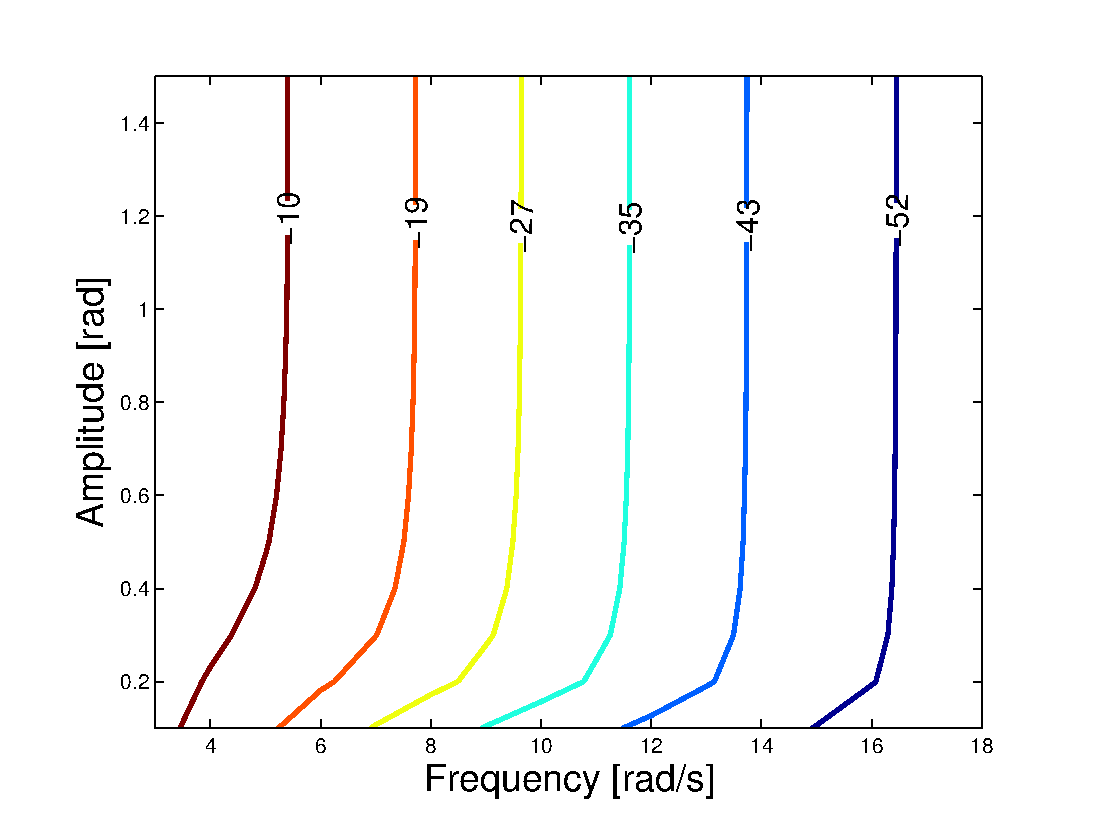
\includegraphics[width=0.5\columnwidth]{dwg/EnergySavingJ1SEA}}
\subfigure[Energy saving in terms of $J_2$ for PEAs.]{\label{fig:EnergySaving_J2_PEA}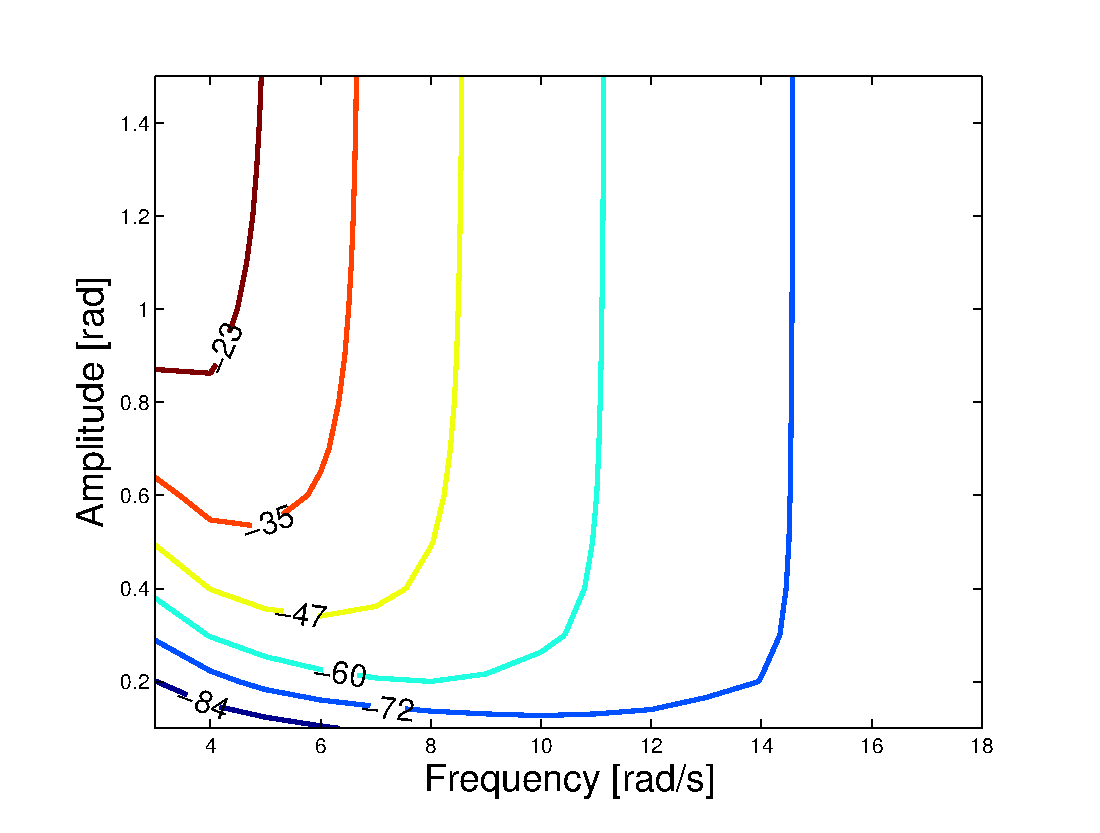
\includegraphics[width=0.5\columnwidth]{dwg/EnergySavingJ2PEA}}
\subfigure[Energy saving in terms of $J_2$ for SEAs.]{\label{fig:EnergySaving_J2_SEA}\includegraphics[width=0.5\columnwidth]{dwg/EnergySavingJ2SEA}}
\caption{Energy saving (in $\%$ w.r.t. the stiff case) for a one-link robot manipulator, varying the amplitude $A$ and the frequency $\omega$ of the desired joint trajectory $q_d(t)=A\sin(\omega t)+B$, with $B=0$.}
\label{fig:EnergySaving}
\end{figure*}

\subsection{One-link Robot manipulator}

First, consider a one-link manipulator, actuated by a SEA or a PEA, which performs a cyclic task. The dynamic of this mechanical system can be written as
\begin{equation}
\begin{aligned}
M\ddot{q} + c\dot{q} + mgL\cos q + K(q-\theta)=0\\
J_{m}\ddot{\theta} + K(\theta-q)=\tau
\end{aligned}
\label{eq:onelinkSEA}
\end{equation}
in case of SEA, and
\begin{equation}
M\ddot{q} + c\dot{q} + mgL\cos q + K(q-q_e)=\tau
\label{eq:onelinkPEA}
\end{equation}
in case of PEA. $M=mL^2+I$, $L$ is the length of the link, $m$ is the load at the end of the link, $I$ the inertia of the link and $c$ is the damping.
Assume that in both cases, the joint trajectory is given as $q_d(t)=B+A\sin(\omega t)$, where the amplitude $A$, the frequency $\omega$, and the angle $B$ around which the link oscillates, depend on the task. 

\paragraph{PEAs} The problem of finding optimal stiffness and pre-load can be solved analytically. Indeed, substituting $q_d(t)$, $\dot q_d(t)$ and $\ddot q_d(t)$ in~\eqref{eq:onelinkPEA}, we can obtain $\tau$
% \[
% \begin{aligned}
% \tau &= A\,M\omega^2\sin(\omega t) + A\,c\,\omega\cos(\omega t) +\\
% &+ mgL\cos(B+A\sin(\omega t)) + K(B+A\sin(\omega t)-q_e)\,.
% \end{aligned}
% \]
and substitute it in $J_1$.
% Let us first consider the cost functional $J_1$ and substitute $\tau$ in it, with $\dot\theta(t)=\dot q(t)$. 
The minimum of $J_1$ is achieved with 
\[
\begin{aligned}
\hat K &= \omega^2 M+\frac{8mgLB_J(2,A)\sin B}{A^2}\\
\hat q_e &= B + \frac{2 g m L A B_J(1,A)\cos B}{A^2\omega^2 M+8mgLB_J(2,A)\sin B}\,,
\end{aligned}
\]
where $B_J(n,x)$ is the Bessel function. Notice that for small amplitudes, i.e.~$A\rightarrow 0$, $\cfrac{8B_J(2,A)}{A^2}\rightarrow 1$, the optimal stiffness becomes $\hat K=\omega^2 M+mgL\sin B$ which corresponds to the resonant condition for the linearized system in $q=B$. % The cost functional in these conditions  becomes
% \begin{equation}
% J_1|_{\hat K,\hat q_e} = A_{PEA}+\pi\frac{A^4 M^2\omega^5-16g^2L^2m^2\omega B_J(1,A)^2}{4}\,.
% \end{equation}
% which is related only on losses due to the damping coefficient.

% Notice that, when $A\rightarrow 0$, i.e. in case of small amplitudes around $q=0$, the optimal stiffness, depending only on $\omega$, does not change whereas the optimal pre-load becomes
% \[
% \hat q_e = \frac{g m L }{\omega^2 M}\,.
% \]
% as the function $\lim_{A\rightarrow 0} B_J(1,\,A)/A=0.5$.
% This result can be obtained considering the linearized system of~\eqref{eq:onelinkPEA} around the point $q=0$ and the optimal stiffness satisfies the resonant condition. As a consequence, the optimal stiffness for the linearized system around $q=0$ is optimal also for the nonlinear system. 

For the cost functional $J_2$, % substituting $q_d(t)$ and its first and second derivative in~\eqref{eq:onelinkPEA}, we have
% \[
% \begin{aligned}
% \tau &= A\,M\omega^2\sin(\omega t) + A\,c\,\omega\cos(\omega t) +\\
% &+ mgL\cos(A\sin(\omega t)) + K(A\sin(\omega t)-q_e)\,.
% \end{aligned}
% \]
% Substituting $\tau$ in the cost functional $J_2$, 
the minimum is obtained with 
\[
\begin{aligned}
\hat K &= \omega^2 M+\frac{2mgLB_J(1,A)\sin B}{A}\\
\hat q_e &= B+\frac{AmgLB_J(0,A)\cos B}{A^2\omega^2 M+2mgLB_J(1,A)\sin B}\,.
\end{aligned}
\]
Also in this case, for small amplitudes, the optimal stiffness becomes $\hat K=\omega^2 M+mgL\sin B$ which corresponds to the resonant condition for the linearized system in $q=B$. % Under these conditions the cost functional can be then rewritten as
% \begin{equation}
% J_2|_{\hat K,\hat q_e} = \pi A^2 c^2 \omega\,,
% \end{equation}
% which is related only to the losses due to the damping coefficient. 
Of course, for the nonlinear system, the cost function obtained by using the optimal parameters assumes a bigger value but $|\tau|$ achieves the minimum value. This is similar to the resonance concept of linear systems.
% This result can be obtained considering the linearized system of~\eqref{eq:onelinkPEA} around the point $q=0$ and the optimal stiffness satisfies the resonant condition. Indeed, this system is a good approximation of the nonlinear one in case of small amplitudes around the origin, i.e.~when $A\rightarrow 0$. Moreover, as the optimal stiffness $K$ obtained for the nonlinear system, depending only on $\omega$, is also optimal for the linearized one, the optimal pre-load value depends also on the amplitude $A$ and for the linearized system becomes 
% \[
% \hat q_e = \frac{g m L}{\omega^2 M}
% \]
% as $\lim_{A\rightarrow 0}B_J(0,A)=1$. 

Finally, for a given $B$, the optimal values for $\hat K$ obtained by using $J_1$ and $J_2$ are quite similar. In particular, if $B=0$ and for any amplitude $A$, $\hat K=\omega^2 M$, i.e.~the value of stiffness corresponding to the resonant condition for the linearized system in $q=0$. The pre-load are different but from a quantitative point of view are quite similar, depending mainly on $B$.

\paragraph{SEAs} The problem of finding optimal stiffness can be solved analytically only in case of $J_2$ as cost functional. Indeed, solving the first equation of \eqref{eq:onelinkSEA} for $\theta$ and substituting it, with its second derivative in the second equation of \eqref{eq:onelinkSEA}, we obtain $\tau$
% \[
% \begin{aligned}
% \tau &= \frac{1}{K}(-A^2 m g L J_m \omega^2 \cos^2(\omega t)\cos(A \sin(\omega t)+B)+\\
% &+A \omega^2 \sin(\omega t) (m g L J_m \sin(A sin(\omega t)+B)+\\
% &-K (M+J_m)+M J_m \omega^2)+ K m g L \cos(A \sin(\omega t)+B)+\\
% &+A d \omega (K-J_m \omega^2) \cos(\omega t))\,.
% \end{aligned}
% \]
and substituting it in $J_2$, with $\dot\theta(t)=K^{-1}(M\ddot q_d(t)+c\,\dot q_d(t)+mgL\cos q_d(t))+q_d(t)$, the minimum can be achieved in closed form. The expression is complicated and can not be reported here. However, in case of $B=0$, $d=0$ and for small amplitudes, the optimal value is
\[
\begin{aligned}
\hat K &= \frac{MJ_m\omega^2}{(M+J_m)}\,,
\end{aligned}
\]
which corresponds to resonant condition for the linearized system around $q=0$, without losses ($d=0$). 

In case of $J_1$, the optimal stiffness and the corresponding value of the cost functional can be only obtained numerically. 
For a comparison between PEA and SEA in terms of efficiency, and to underline the advantage of soft w.r.t.~stiff actuation, in Fig.~\ref{fig:EnergySaving} we report the cost saving in terms of $J_1$ and $J_2$ in case of PEAs or SEAs w.r.t. the stiff case. In particular, Fig.~\ref{fig:EnergySaving_J1_PEA} and \ref{fig:EnergySaving_J1_SEA} show the energy saving using $J_1$ as measure. On the other hand, Fig.~\ref{fig:EnergySaving_J2_PEA} and \ref{fig:EnergySaving_J2_SEA} show the energy saving using $J_2$ as measure.

In particular, considering Fig.~\ref{fig:EnergySaving_J1_PEA} and \ref{fig:EnergySaving_J2_PEA}, the use of PEAs permit to get as much more saving as the amplitude and the frequency of the desired trajectory decrease, independently from the cost functional used, i.e.~$J_1$ or $J_2$. However, we have a consistent saving also in case of large values of frequency, independently from the amplitude. 

Differently, in case of SEA, savings depend on the cost functional we consider. In terms of $J_1$, consistent savings can be obtained increasing the frequency. The amplitude significantly influence only for small values. In terms of $J_2$, consistent savings can be obtained for small values of the amplitude and large values of frequency or for large values of the amplitude and small values of frequency. 

From another point of view, we can conclude that, in terms of $J_2$, PEA is more convenient for small amplitudes at low frequency or large amplitudes at high frequency, while SEA is more convenient for small amplitudes at high frequency or for large amplitudes at low frequency. In terms of $J_1$, we can observe differences w.r.t. $J_2$ only in case of SEA. Indeed, SEA becomes convenient only for high frequencies, independently from the amplitude.
% \begin{figure}[!t]
% \centering
% 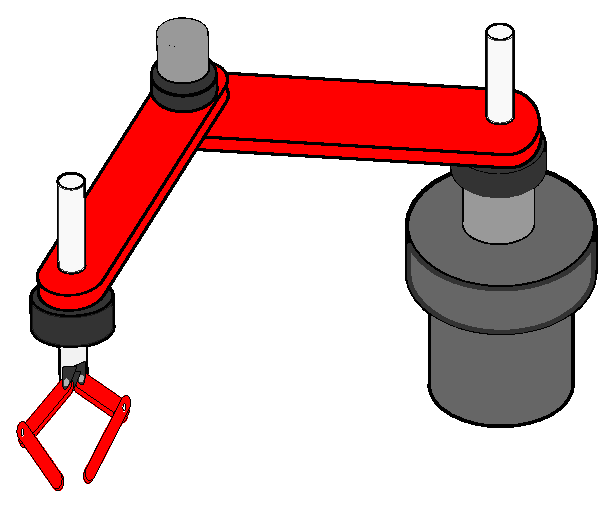
\includegraphics[width=0.6\columnwidth]{dwg/scara}
% \caption{Two-DoF robot Manipulator for a pick and place task.}
% % With, $m = 0.840 \ [kg]; \ l_1 = 0.140 \ [m]; \ l_2 = 0.165 \ [m]; \ l = 0.055 \ [m]$
% \label{fig:scara}
% \end{figure}
%%-%
\begin{figure*}[!t]
\centering
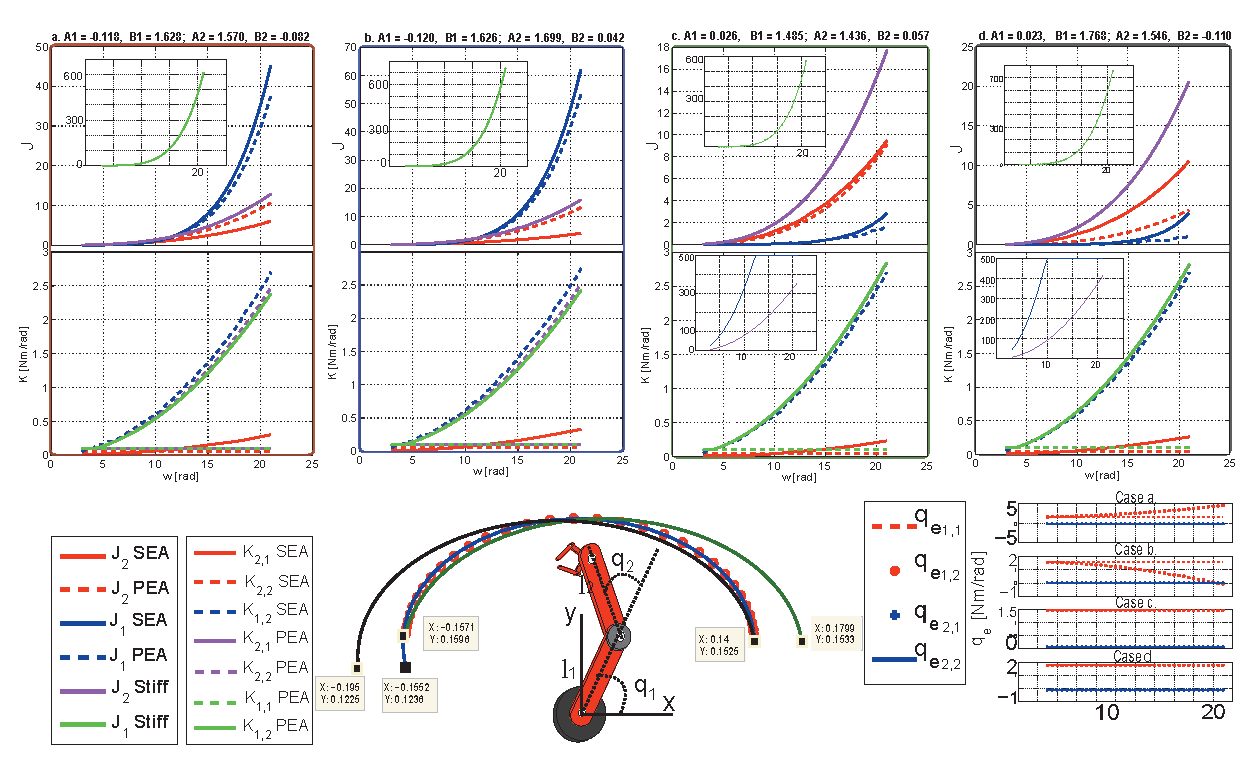
\includegraphics[width=0.88\textwidth]{dwg/TwoLinksManipulator}
\caption{The dynamics parameters used are: link masses $m_1 = m_2 = 0.84$~kg; link lengths $l_1 = 0.14$~m, $l_2 = 0.165$~m; motor inertias $J_{m_{1}} = J_{m_{2}} = 10^{-5}$~$kg m^2$, link inertias motor inertias $J_1 = 3.96\,10^{-4}$~kgm$^2$ $J_2 = 5.29\,10^{-4}$~kgm$^2$ w.r.t. centroid. The red, blue, green and black curves on the center of the figure show the desired end-effector trajectories. The corresponding results of cost functionals and optimal stiffness are shown in the boxes of the same color (a. to d. from left to right). The figure legends are indicated below the boxes. For cases a. and b. (red and blue), $\hat K_{(1,1)SEA} = \ 500 \ Nm/rad$ so it is not shown; for cases c. and d. (green and black) it is indicated with blue continuous line. The pre-load optimization results for the PEA case are shown at bottom right.}
\label{fig:PickAndPlace}
\end{figure*}

\subsection{Two--link robot manipulator}

Let us consider now a two-link robot manipulator which performs a pick and place task. The robot moves on a horizontal plane.
% and hence the dynamic, in case of PEAs, is
% \[
% \dots
% \]
% where $q_1$ and $q_2$ are the link positions, $\ell_1$ and $\ell_2$ the length of each link, $J_1$ and $J_2$ their inertias and $\tau_1$ and $\tau_2$ the torques generated by motors. In case of SEAs, we have
% 
% 
% where $\theta_1$ and $\theta_2$ the motor positions. 
In case of PEAs, we have a fully actuated mechanical system (2 motors and 2 DoFs), whereas in case of SEAs an under-actuated one (2 motors and 4 DoF). $q_{1,d}=A_1\sin(\omega t)+B_1$ and $q_{2,d}=A_2\sin(\omega t)+B_2$ are the desired joint trajectories. The robot moves from a given initial position $Q_1$ to a given final position $Q_2$. The values of the amplitudes $A_1$ and $A_2$, as well as the angle $B_1$ and $B_2$ around which each link moves, depend on these positions. Of course, for any couple of point $Q_1$ and $Q_2$, these parameters are univocally determined by inverse kinematics.
% the desired end-effector trajectory is
% \[
% \begin{aligned}
% 	x_{e,d} &= \ell_1\cos q_{1,d}+\ell_2\cos(q_{1,d}+q_{2,d})\\
% 	y_{e,d} &= \ell_1\sin q_{1,d}+\ell_2\sin(q_{1,d}+q_{2,d})\,,
% \end{aligned}
% \]
% and hence, 
% \[
% \rho_{e,d}=\sqrt{\ell_1^2+\ell_2^2+2\ell_1\ell_2\cos q_{2,d}}
% \]
For this problem, we have performed several simulations applying our methodology. Some of them are reported in Fig.~\ref{fig:PickAndPlace}, which shows the values of cost functionals $J_1$ and $J_2$ in case of PEAs and SEAs, as well as the optimal parameters (stiffness and/or pre-load) for different values of frequency $\omega$. Moreover, cost functionals $J_1$ and $J_2$ for the same tasks for the stiff case are also reported. Notice that for all cases reported in Figure~\ref{fig:PickAndPlace}, the cost functionals assume the minimum values. % and $A_1\equiv A_2$.

For all cases, it is shown in Fig.~\ref{fig:PickAndPlace} that the stiff actuation is the most expensive in terms of energy spent. Furthermore, in the first two cases (a. and b.), when using $J_1$, PEA gives the lowest cost, while for the other two cases (c. and d.) the best performance is achieved when using SEA. The same happens for $J_2$. The optimal joint stiffness is higher as $\omega$ increases.
Moreover, for the SEA case, the spring in the first joint should be stiffer than the second joint, while for the PEA case, the spring for the first joint should be softer than the second one. Results evidence that elastic actuators allow to save energy. Indeed, at the highest frequency used in these simulations, the energy savings in terms of cost functional $J_1$ is up to $90\%$ w.r.t.~the rigid case in the SEA and PEA cases. In terms of $J_2$, at the same frequency, the energy savings is up to $62\%$ in case of SEAs and $23\%$ in case of PEAs, w.r.t.~the rigid case. In Fig.~\ref{fig:PickAndPlace} is also reported values of the optimal pre-load values $q_e$ for the PEA case. Notice that this value is constant for all cases except for the cases a. and b. where the optimal pre-load value of the second joint changes with frequency.

% For all cases, it is shown in Figure~\ref{fig:PickAndPlace} that using $J_1$, the stiff actuation is the most expensive in terms of energy spent, as well as when using $J_2$. Furthermore, for both indices $J_1$ and $J_2$, SEA provides the best performance. For the red and blue curves, and considering the range $\omega \in  \ [3, \ 15]$~rad/s, $J_1$ values in the PEA case are quite similar to those related to the same cost functional but in the SEA case. For higher frequencies, results show that it would be better to use PEA.
% On the other hand, for all cases, the optimal joint stiffness is higher as $\omega$ increases. Moreover, for the SEA case, the first joint should be stiffer than the second joint, while for the PEA case, the first joint should be softer than the second one. Results suggest that in general, elastic actuators allow to save energy; for PEA, $J_2$ is lower, whereas for SEA, $J_1$ has the lowest values. The corresponding joint stiffness are softer than those obtained by using $J_1$ for PEA and $J_2$ for SEA.

%!TEX root = Humanoids2013.tex
\section{Model--Free Application}

In this section we present an experimental application on a prototype of the hopping robot represented in Fig.~\ref{fig:Prototype}. The objective is to show that, even though the proposed method is analytical, it is directly applicable to existing systems whose model is not accurate or not available at all. Indeed, the optimization of the actuation parameters need to evaluate the function $f_a(\ddot x, \dot x, x, \ddot{q}, \dot{q}, q, t)$ and in~\eqref{eq:underact1_SEAplus} in case of SEA, or in \eqref{eq:underact_PEAplus} in case of PEA, in terms of the desired joint trajectories. However, in an experimental setup, as $f_a(\cdot)$ can also be directly measured from the real system by means of suitable sensors.  
To correctly the optimization procedure, it is sufficient to obtain the derivatives of the measured signal $f_a(t)$, which can be obtained by applying techniques such as e.g.~in~\cite{Fliess2003}.
Through the following experiment we are hence able to show that our method can be applied to systems whose model is unknown, i.e.~in a model--free fashion. 

% The procedure proposed in this paper is applied to the prototype of the hopping robot represented in Fig.~\ref{fig:Prototype} mainly to show that, nonetheless the method is based on the knowledge of the model of the mechanical system, it works well also using experimental data acquired directly from sensors suitable placed on the real system, i.e.~in a model--free fashion. 

The prototype of the planar elastic hopping robot represented in Fig.~\ref{fig:Prototype}. Referring to Fig.~\ref{fig:SaltarelloEsploso}, it has one leg which is composed of two links (1 and 2), three DoFs and it is linked to the frame through two non actuated DoFs  (3 and 4). All joints are provided with a contactless magnetic rotary position sensor (AS5045\footnote{\url{http://www.ams.com}}, colored in red). The two joints of the leg are actuated by DC geared motors (maxon DCX 22S\footnote{\url{http://dcx.maxonmotor.com}} with graphite brushes $24$ V, and planetary gearhead GPX22 with reduction ratio $83:1$, 5 and 6). The hopper is actuated by a SEA in the knee, while the other joint is stiff (see Fig.~\ref{fig:SaltarelloEsploso}).
The series elastic transmission 10 between the actuator 11 and the knee joint is composed of two rubber bands. 

Wheel 7 is placed at the extremity of the leg in order to reduce the effect of the friction component perpendicular to the direction of motion. To guarantee a vertical hopping, the leg has been constrained through a vertical linear guide 8. An electronic board\footnote{\url{http://www.naturalmotioninitiative.com/}} 9 has been used to acquire the measurements from the encoders and to implement a closed loop position control scheme tracking the desired trajectories (the controller furnishes input values at a frequency of $1$ kHz).
\begin{figure*}[!t]
\centering
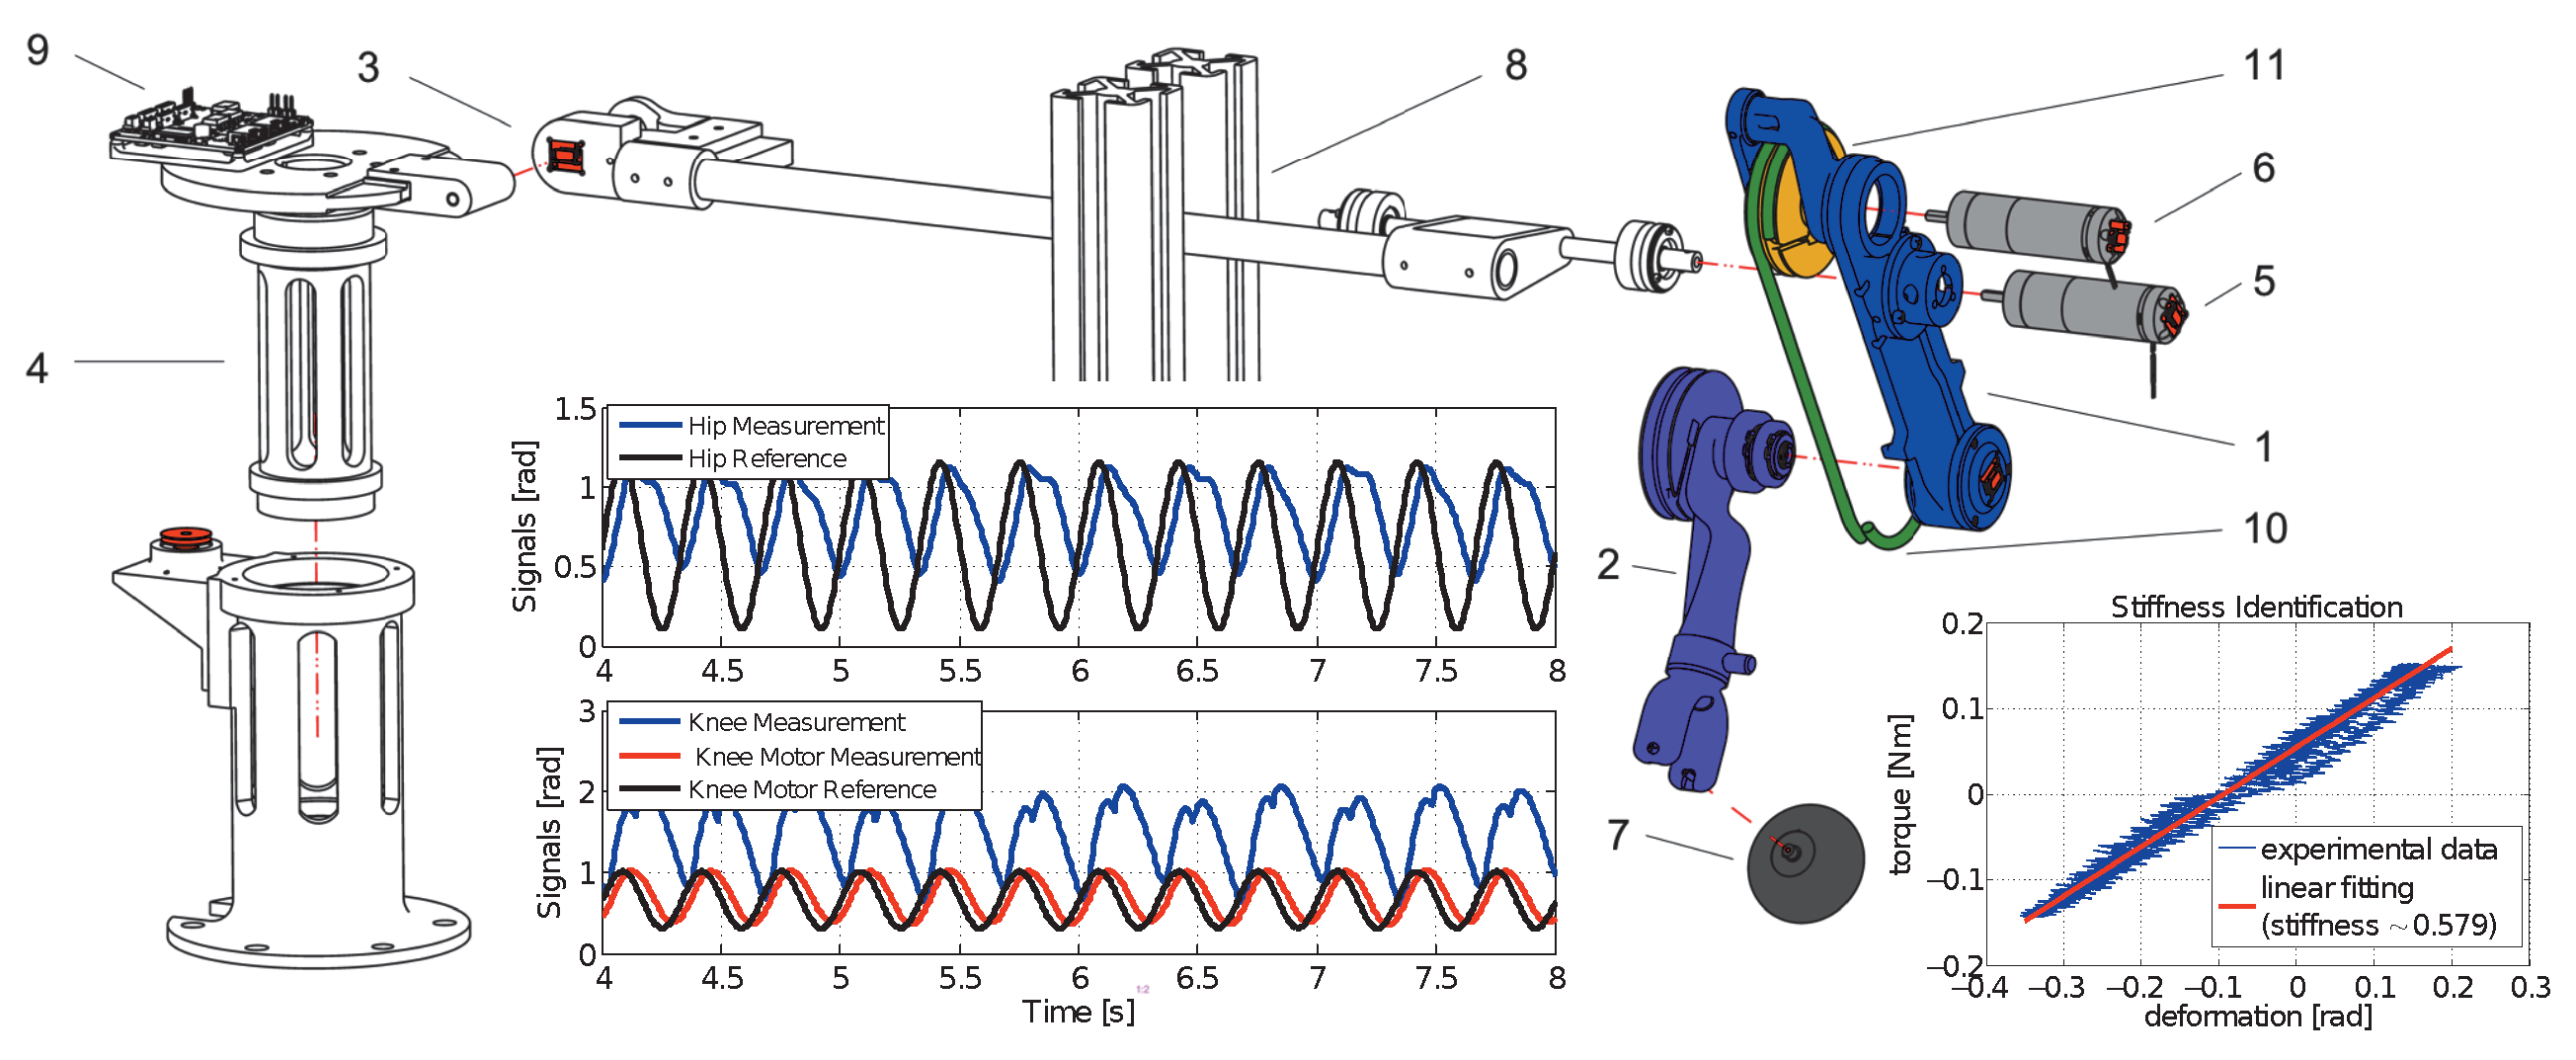
\includegraphics[width=0.89\textwidth]{dwg/SaltarelloEsploso}
\caption{Exploded 3D view of the hopping robot. The figure also shows the graphical values of torque and corresponding deformation used for stiffness identification. Moreover, in the center of the picture are reported reference signals and measured link trajectories.}
\label{fig:SaltarelloEsploso}
\end{figure*}

% \begin{figure}[!t]
% \centering
% \includegraphics[width=0.9\columnwidth]{dwg/curveJ1pea}
% \caption{.}
% \label{fig:SaltarelloEsploso}
% \end{figure}
% 
% \begin{figure}[!t]
% \centering
% 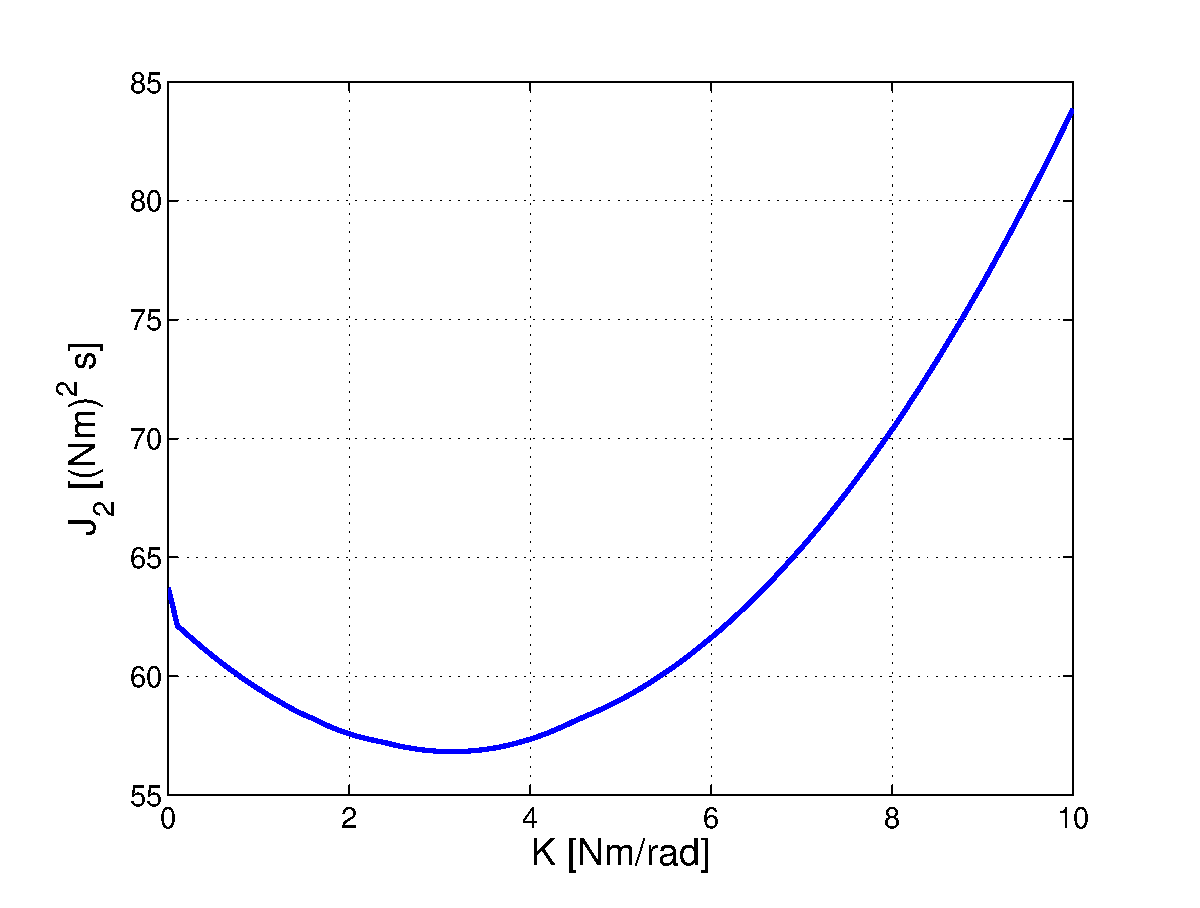
\includegraphics[width=1\columnwidth]{dwg/curveJ2pea}
% \caption{.}
% \label{fig:SaltarelloEsploso}
% \end{figure}

%%-%
\begin{figure*}[t]
\centering
\subfigure[Cost index $J_2$ for different values stiffness in case of SEAs.]{\label{fig:J2_SEA}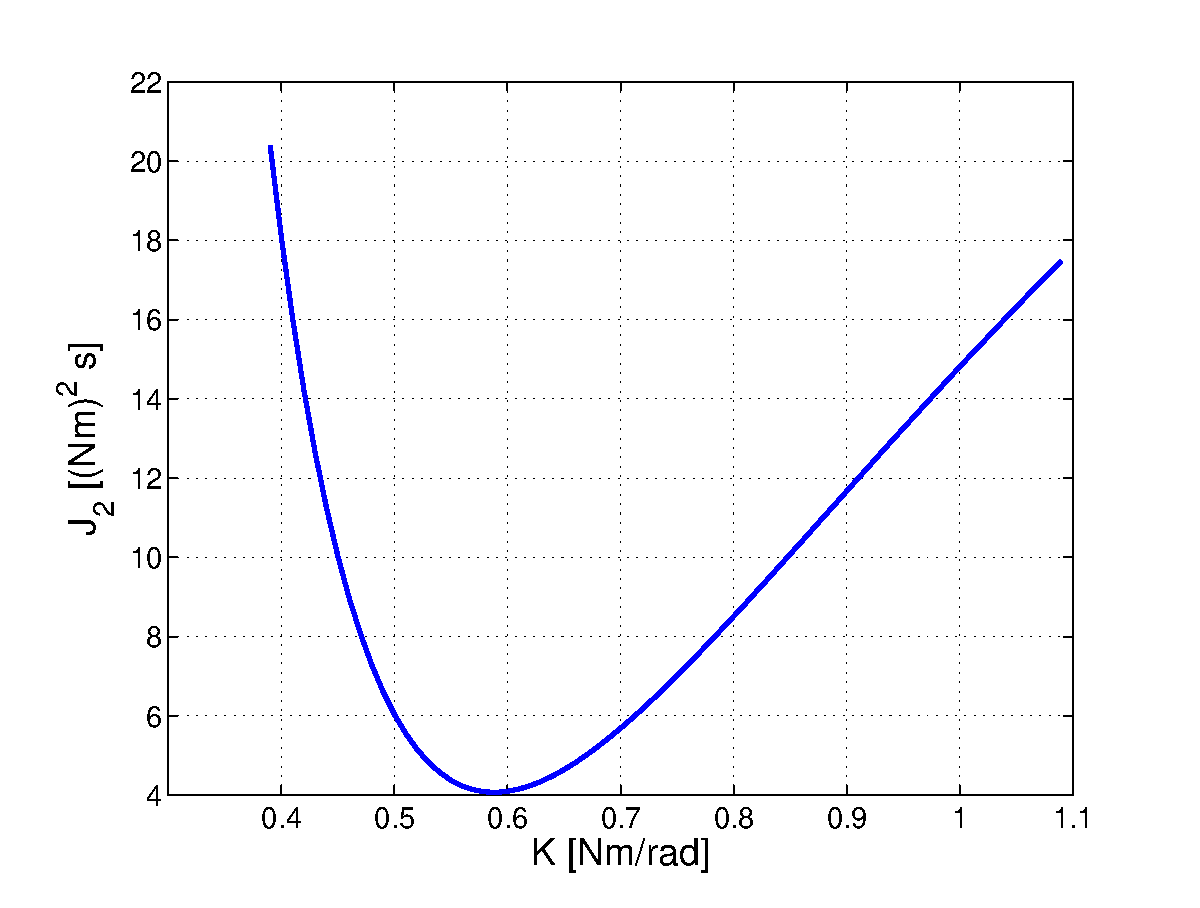
\includegraphics[width=0.5\columnwidth]{dwg/curveJ2sea}}
\subfigure[Cost index $J_2$ for different values stiffness in case of PEAs.]{\label{fig:J1_PEA}\includegraphics[width=0.5\columnwidth]{dwg/curveJ1pea}}
\subfigure[Cost index $J_1$ for different values stiffness in case of SEAs.]{\label{fig:J1_SEA}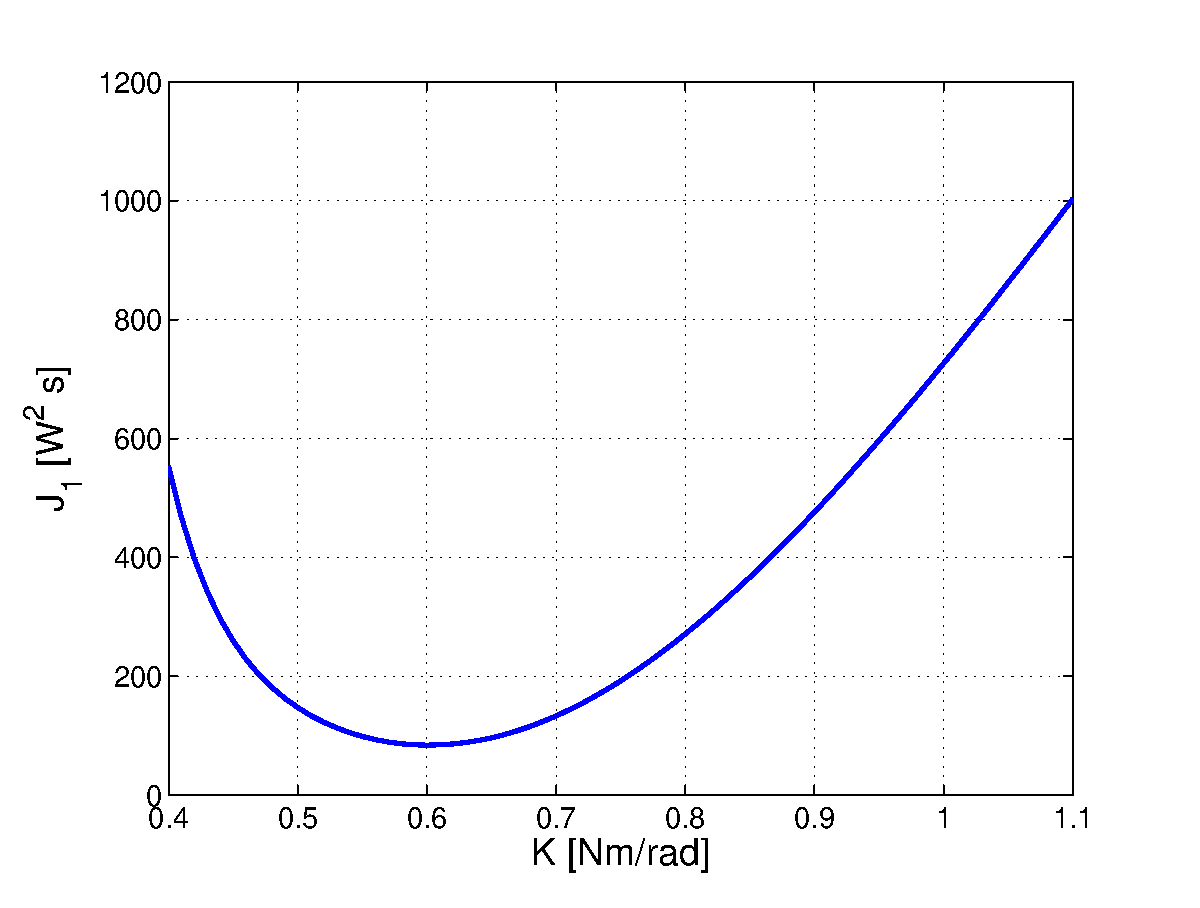
\includegraphics[width=0.5\columnwidth]{dwg/curveJ1sea}}
\subfigure[Cost index $J_1$ for different values stiffness in case of PEAs.]{\label{fig:J2_PEA}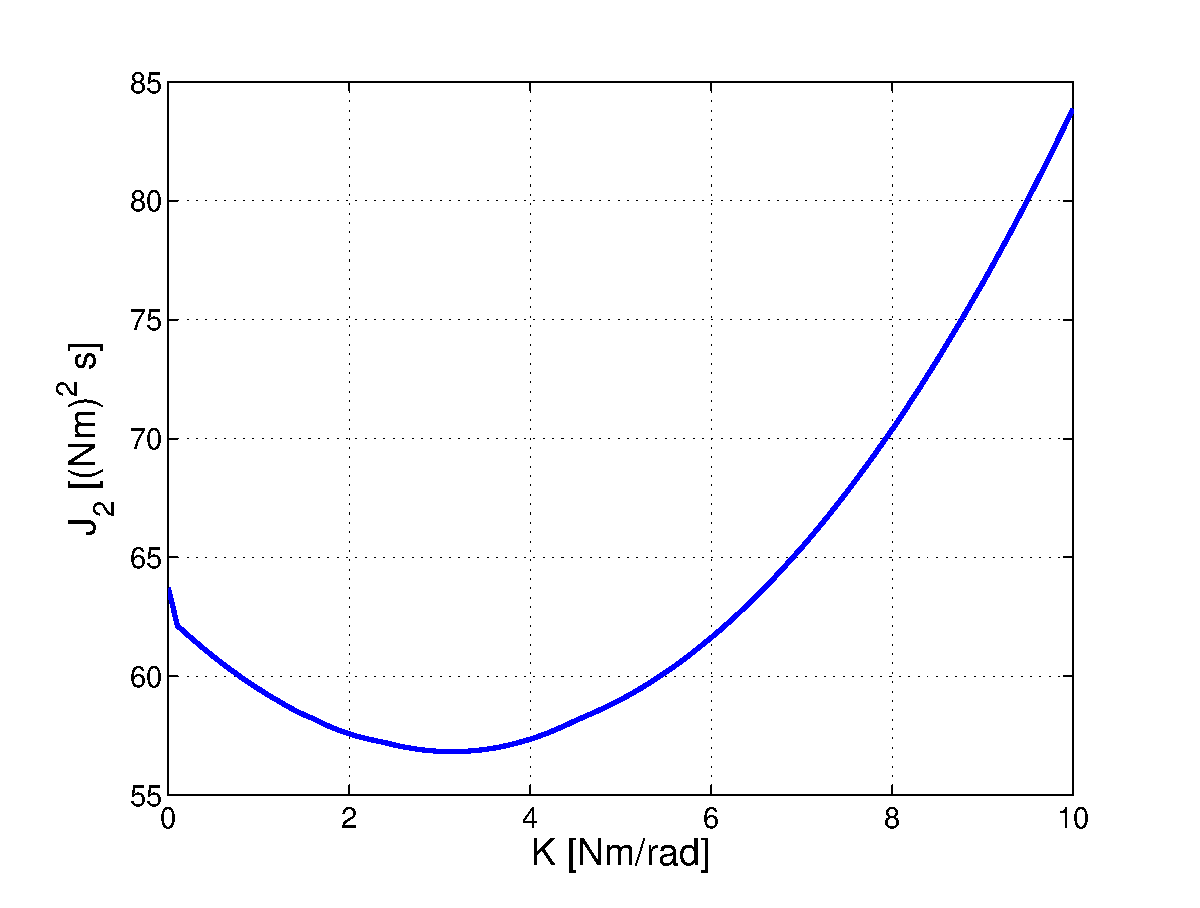
\includegraphics[width=0.5\columnwidth]{dwg/curveJ2pea}}
\caption{Cost indices $J_1$ and $J_2$ for different values of $K$. In the PEA case, for each value of stiffness, the corresponding value of the cost functional is computed by using the best value of $\hat q_e$.}
\label{fig:CostSaltarello}
\end{figure*}

% In order to demonstrate that our method can be applied in a model--free 
% 
% carry out experiments, we apply our methodology to the mechanical model of the hopping robot to find the optimal actuation parameters.
The stiffness of the equivalent torsional spring between the knee link and the actuator has been experimentally determined by applying different value of torques and the corresponding deformations (see Fig.~\ref{fig:SaltarelloEsploso}, Stiffness identification). Once the stiffness value is known ($\sim0.58$~Nm/rad), sinusoidal reference signals that guarantee a stable hopping have been imposed to the motors (black lines in Fig.~\ref{fig:SaltarelloEsploso}). During the experiment (see the attached video), we have recorded data provided by encoders (red and blue lines in Fig.~\ref{fig:SaltarelloEsploso}), and hence the signal $f_a(t)$ in~\eqref{eq:underact1_SEAplus} in case of SEA, or \eqref{eq:underact_PEAplus} in case of PEA. Having the signal $f_a(t)$, it is possible to apply our method to determine, for those link trajectories, the values of cost functional $J_1$ and $J_2$ for different values of $K$ and, for PEA, the corresponding best value of $q_e$, as reported in Fig.~\ref{fig:CostSaltarello}.

% The experiment is conducted as follows: (i) the stiffness of the equivalent torsional spring between the knee joint and the actuator has been experimentally determined (see Fig.~\ref{fig:SaltarelloEsploso}); (ii) sinusoidal references giving a stable hopping has been provided to the motors;
% % (stability has been evaluated by letting the experiment go until the signals become stable loop); 
% (iii) through the motor and link positions provided by sensors, the torque furnished by the motor has been evaluated; (iv) our algorithm has been applied to optimize the spring stiffness.


% Figure~\ref{fig:CostSaltarello} shows the values of indices $J_1$ and $J_2$ for different values of stiffness assuming that the hopper is actuated by PEAs and SEAs. 
For both indices the best result in terms of energy saving can be obtained for $SEAs$ by setting $K\approx 0.6$~Nm/rad as stiffness value. 
% The experimental tests has been conducted as follows:
% \begin{itemize}
%       \item the stiffness of the equivalent torsional spring between the knee joint and the actuator has been experimentally determined (see Fig. [TODO FIG REF])
%       \item sinusoidal references giving a stable hopping (stability has been evaluated by letting the experiment go until the signals become stable loop) has been provided to the motors
%       \item through the motor and link measured position the torque exerted by the motor has been evaluated
%       \item the algorithm has been applied to optimize the spring
% \end{itemize}
% We have set this optimal stiffness value on the prototype with given joint trajectories which correspond to sinusoidal signals. As shown in Fig.~\ref{fig:SaltarelloEsploso}, the real value of stiffness set to the joint is $K\approx 0.58$~Nm/rad, quite similar to the optimal one.  
Notice that, this value is quite similar to that obtained by the stiffness identification procedure. Hence, if the controller is able to guarantee the same joint trajectories used in the optimization phase, with any other value of stiffness, the energy spent would increase.


% In Fig.~\ref{fig:SaltarelloEsploso} the desired references for the knee and hip joint trajectories (black curve) and the corresponding measured link (blue curve) and motor (red curve) trajectories. Notice that, , due to SEA actuation, for the knee, the link trajectory can be different from the motor trajectory which is  
% 
% 
%   the   of the reference signls for the hip and the knee motor is also reported.

% \subsection{Underactuated Mechanical system: Hopping Robot with PEAs}
% 
% In order to demonstrate the effectiveness and application of our method, we apply it to a prototype of 
% 
% A two link hopper is then projected to evaluate the algorithm exposed in the precedent sections. The model is a 4 D.o.F. with the first two under actuated to implement the floating base model and the last two actuated to implement the jump. The system is composed by two links presenting the first and second anatomic part of a leg \(Femur\; and\; Tibia\), a wheel for the contact point, two DC motors ,two pulleys, two elastic tendons and a base support to constraints the system. It is also present the necessary electronics for the communication. The major parts of the model are specifically designed and printed with a fast prototyping 3d printer.\\ 
% 
% The floating base is implemented as a base support which is composed by a vertical rolling cylindric structure jointed to a horizontal tube, which connects the hopper to the base implementing the second D.o.F. The base support constraints the hopper to move in the sagittal plane. At the end of the tube a motor is placed to implement the hip D.o.F. then the first link is mounted on the shaft. On the top of the same link is placed the motor to implement the knee D.o.F. which transmits the movement to the respective joint considering a transmission composed by pulleys and tendon obtaining a SEA actuator. The second link is then connected to the first by a rotoidal joint and a wheel is mounted at the end to implement a point of contact. The axle of the wheel is normal to the tube to allow .... in the radial direction of the base support. An additional material is posed on the wheel's surface to improve the constant of friction in the contact between the ground and the wheel. The Hopper is then constrained to provide a steady jump constraining the tube which connect the hopper to the base support. The complete structure is presented in fig. \ref{fig:}.
%  
% \subsubsection{Experimental setup}
% 
% \paragraph{Electronics and Interface}
% 
% From the electrical point of view, every actuated and no actuated joint presents an encoder which is connected by bus to a SCHEDINA.... The SCHEDINA handles the power supply of the motor and the communication. The control is open loop considering a low proportional gain on \\
% schedina di bons\\
% controllo in anello aperto\\
% proporzionale du motore\\\\
% tempo trasmissione\\
% gioco sulle interruzioni e altre cose che ha fatto lore\\
% 
% \subsection{Results}
% 
% The system is first implemented in Adams to find a reasonable set of sinusoidal signals necessary to jump. Reasonable ground contact parameters are used to have a realistic simulation and the analog rotoidal stiffness of the SEA on the Knee is estimated too. The signals imposed to the simulator are sinusoidal at the same frequency and variations of its module, the amplitudes and the bias are studied. This set is then implemented by software and tested on the system. Then the measurements obtained by the experiments are processed by the algorithm presented above. The results are presented in table \ref{} which shows the functional cost and the stiffness calculated. To validate ... 
%!TEX root = Humanoids2013.tex
\section{Conclusions and future work}

In this paper, we have studied the role of soft actuation in the reduction of the energy cost for mechanical systems that perform cyclic tasks. We have considered both SEAs and PEAs and determined the optimal stiffness value and spring pre-load such that a given cost functional is minimized. We have shown that the energy consumption also depends on the shape of the joint trajectories used to perform a given cyclic task. In this paper the desired joint trajectories are sinusoids which may not guarantee the best behavior in terms of energy saving. Future works will be dedicated to explore the role of the shape of the joint trajectories in the reduction of the energy cost as well as how to design them.

Moreover, results obtained in this paper can be applied directly to more complex systems such as hopping or humanoid robots for which soft actuation can be exploited to achieve a reduction of the the so called ``Cost of Transport'' which is an important aspect of these robots. Future works will be dedicated to show by experimentation the reduction of the energy consumption.

\section{Acknowledgment}
Authors gratefully acknowledge Felipe Belo, Fabio Bonomo, Manuel Giuseppe Catalano, Manuel Bonilla, Kamilo Melo, Alessandro Serio and Andrea Di Basco for their assistance in the prototype design.



\bibliographystyle{IEEEtran}
\bibliography{IEEEabrv,Biblio}

\end{document}
